\documentclass[amscd, amssymb, verbatim]{amsart}[12pt]

\usepackage{fullpage}
\usepackage{amssymb}
\usepackage{latexsym}
\usepackage{pb-diagram}
\usepackage[mathscr]{euscript}
\usepackage{graphicx}
\usepackage{subfigure}
\usepackage{placeins}
\usepackage{wrapfig}
\usepackage{hyperref}
\usepackage{appendix}
\usepackage{multind}
\usepackage{natbib}
\bibpunct{[}{]}{;}{a}{}{,~}

\theoremstyle{remark}
\newtheorem{exercise}{Exercise}
\theoremstyle{remark}
\newtheorem{exerciseSol}{Exercise}
\theoremstyle{remark}
\newtheorem*{solution}{Solution}

\DeclareMathOperator{\VR}{VR}
\DeclareMathOperator{\W}{W}
\DeclareMathOperator{\LW}{LW}

\begin{document}

\title{javaPlex Tutorial}

\author{Henry Adams}
\email[H.~Adams]{henrya@ima.umn.edu}

\author{Andrew Tausz}
\email[A.~Tausz]{andrew.tausz@gmail.com}

\date{\today}

\maketitle

\tableofcontents
\setlength{\parindent}{0pt}
\setlength{\parskip}{8pt}

% TODO:  Move dump example up to earlier section of tutorial?

% TODO: test tutorial after making changes to include examples finding representative cycles (For example, getDefaultSimplicialAlgorithm changed everywhere to getModularSimplicialAlgorithm).

% TODO: Add more figures with data points in blue and landmarks in red, such as the one in exercise_19, to this tutorial.

% TODO: the figures for the random trials in this tutorial don't currently match the numbers (number of simplices, etc).
%UPDATE: They do for witness_example.m and lazy_witness_example.m

% "Googlecode Issue": Add primary circle and three circle natural image examples to the tutorial. In particular, these are good examples of how different core subsets can produce different topologies.

% "Googlecode Issue": In the tutorial, explain the new feature that allows the user to specify the initial seed used for sequential maxmin landmark selection. This feature has been added as a result of  Issue 23  (fixed).

% TODO: explain API class and how most commands for users are in this class (API does not contain under-the-hood implementation, but instead shows what the user can do w/ the library.) Check if Lazy Witness is in API; if not, perhaps it should be added.

% TODO: add example which is FLAT double torus. That is, select points at random from an octagon. Then, create explicit metric by identifying sides.
% UPDATE: added example for double torus embedded in R^3.

% TODO: is "ensureAllFaces" working as I expect? See representatives_example_HA and try changing dimensions.
% UPDATE: See javaplex Issue 20 created by Andrew.

% TODO: add exercise numbers to tutorial wiki.

% TODO: Add zigzag examples to tutorial. See:
% http://code.google.com/p/javaplex/source/browse/#svn%2Ftrunk%2Fsrc%2Fmatlab%2Fexperimental%2Fvietoris_rips_bootstrap
% http://code.google.com/p/javaplex/source/browse/#svn%2Ftrunk%2Fsrc%2Fmatlab%2Fexperimental%2Fwitness_bootstrap
% http://arxiv.org/abs/1108.3545
% Also, see email from Anthony Bak 10-21-11

% TODO: ask Andrew: Move lazy witness to API so that the syntax is more similar to Vietoris-Rips and witness filtrations?




\section{Introduction}


\subsection{javaPlex}

javaPlex is a Java software package for computing the persistent homology of filtered chain complexes, with special emphasis on applications arising in topological data analysis. The main author is Andrew Tausz. javaPlex is a re-write of the JPlex package, which was written by Harlan Sexton and Mikael Vejdemo Johansson. The main motivation for the development of javaPlex was the need for a flexible platform that supported new directions of research in topological data analysis and computational persistent homology. The website for javaPlex is \url{http://javaplex.github.io/javaplex/}, the documentation overview is at \url{https://github.com/javaplex/javaplex/wiki/Overview}, and the javadoc tree for the library is at \url{http://javaplex.github.io/javaplex/doc.4.2.0/}.

This tutorial is written for those using javaPlex with Matlab. However, one can run javaPlex without Matlab; see \url{https://github.com/javaplex/javaplex/wiki/Interoperability}.

If you are interested in javaPlex, then you may also be interested in the software package Dionysus by Dmitriy Morozov (\url{http://www.mrzv.org/software/dionysus}) or the software package Persus by Vidit Nanda (\url{http://www.sas.upenn.edu/~vnanda/perseus/index.html}).

Some of the exercises in this tutorial are borrowed from Vin de Silva's {\em Plexercises}, available at \url{http://comptop.stanford.edu/u/programs/Plexercises2.pdf}.

Please email Henry at \texttt{henrya@ima.umn.edu} or Andrew at \texttt{andrew.tausz@gmail.com} if you have questions about this tutorial.


\subsection{License}

javaPlex is an open source software package under the Open BSD License. The source code can be found at \url{https://github.com/javaplex/javaplex}.


\subsection{Installation for Matlab}
Open Matlab and check which version of Java is being used. In this tutorial, the symbol \texttt{>>} precedes commands to enter into your Matlab window.

\begin{quote} \begin{verbatim} 
>> version -java
ans = Java 1.5.0_13 with Apple Inc.   Java Hotspot(TM) Client VM mixed mode, sharing
\end{verbatim} \end{quote}

javaPlex requires version number \texttt{1.5} or higher. 

To install javaPlex for Matlab, go the the website \url{https://github.com/javaplex/javaplex/tree/master/dist}. Download the zip file containing the Matlab examples. It should be called something like \texttt{matlab-examples\-4.2.0.tar.gz}. Extract the zip file. The resulting folder should be called \texttt{matlab\_examples}.

Change directories in Matlab to \texttt{matlab\_examples}. Run the \texttt{load\_javaplex.m} file. 

\begin{quote} \begin{verbatim} 
>> load_javaplex
\end{verbatim} \end{quote}

Installation is complete. Confirm that javaPlex is working properly with the following command.

\begin{quote} \begin{verbatim}
>> api.Plex4.createExplicitSimplexStream()
ans = edu.stanford.math.plex4.streams.impl.ExplicitSimplexStream@513fd4
\end{verbatim} \end{quote}

Your output should be the same except for the last several characters. Each time upon starting a new Matlab session, you will need to run \texttt{load\_javaplex.m}.


\subsection{Java heap size}
Depending on the size of your javaPlex computations, you may need to increase the maximum Java heap size. This should not be necessary for the examples in this tutorial.

The following command returns your maximum heap size in bytes.
\begin{quote} \texttt{>> java.lang.Runtime.getRuntime.maxMemory\\
ans = 130875392
} \end{quote}
My Matlab installation sets the limit to approximately 128 megabytes by default. To increase your limit to, say, 1.5 gigabytes, create a file named \texttt{java.opts} in your Matlab directory which contains the text \texttt{-Xmx1500m} and then restart Matlab. For more information, please see this link: \url{http://www.mathworks.com/support/solutions/en/data/1-18I2C/}.


\subsection{Accompanying files}

The following Matlab scripts containing the commands in this tutorial are available in the folder \href{https://github.com/javaplex/javaplex/tree/master/src/matlab/for_distribution/tutorial_examples}{\texttt{tutorial\_examples}}. This means that you don't need to type in each command individually.
% Add note? DONT copy and paste commands from pdf
\begin{itemize}
\item \href{https://github.com/javaplex/javaplex/tree/master/src/matlab/for_distribution/tutorial_examples/bottleneck_distance_example.m}{\texttt{bottleneck\_distance\_example.m}}
\item \href{https://github.com/javaplex/javaplex/tree/master/src/matlab/for_distribution/tutorial_examples/core_subsets_example.m}{\texttt{core\_subsets\_example.m}}
\item \href{https://github.com/javaplex/javaplex/tree/master/src/matlab/for_distribution/tutorial_examples/euler_characteristic_example.m}{\texttt{euler\_characteristic\_example.m}}
\item \href{https://github.com/javaplex/javaplex/tree/master/src/matlab/for_distribution/tutorial_examples/explicit_metric_space_example.m}{\texttt{explicit\_metric\_space\_example.m}}
\item \href{https://github.com/javaplex/javaplex/tree/master/src/matlab/for_distribution/tutorial_examples/explicit_simplex_example.m}{\texttt{explicit\_simplex\_example.m}}
\item \href{https://github.com/javaplex/javaplex/tree/master/src/matlab/for_distribution/tutorial_examples/house_example.m}{\texttt{house\_example.m}}
\item \href{https://github.com/javaplex/javaplex/tree/master/src/matlab/for_distribution/tutorial_examples/image_patch_example.m}{\texttt{image\_patch\_example.m}}
\item \href{https://github.com/javaplex/javaplex/tree/master/src/matlab/for_distribution/tutorial_examples/landmark_example.m}{\texttt{landmark\_example.m}}
\item \href{https://github.com/javaplex/javaplex/tree/master/src/matlab/for_distribution/tutorial_examples/lazy_witness_example.m}{\texttt{lazy\_witness\_example.m}}
\item \href{https://github.com/javaplex/javaplex/tree/master/src/matlab/for_distribution/tutorial_examples/pointcloud_example.m}{\texttt{pointcloud\_example.m}}
\item \href{https://github.com/javaplex/javaplex/tree/master/src/matlab/for_distribution/tutorial_examples/rips_example.m}{\texttt{rips\_example.m}}
\item \href{https://github.com/javaplex/javaplex/tree/master/src/matlab/for_distribution/tutorial_examples/witness_example.m}{\texttt{witness\_example.m}}
\end{itemize}
The folder \href{https://github.com/javaplex/javaplex/tree/master/src/matlab/for_distribution/tutorial_examples}{\texttt{tutorial\_examples}} also contains the following Matlab functions
\begin{itemize}
\item \href{https://github.com/javaplex/javaplex/tree/master/src/matlab/for_distribution/tutorial_examples/coreSubset.m}{\texttt{coreSubset.m}}
\item \href{https://github.com/javaplex/javaplex/tree/master/src/matlab/for_distribution/tutorial_examples/dct.m}{\texttt{dct.m}}
\item \href{https://github.com/javaplex/javaplex/tree/master/src/matlab/for_distribution/tutorial_examples/eulerCharacteristic.m}{\texttt{eulerCharacteristic.m}}
\item \href{https://github.com/javaplex/javaplex/tree/master/src/matlab/for_distribution/tutorial_examples/kDensitySlow.m}{\texttt{kDensitySlow.m}}
\end{itemize}
and the following Matlab data files
\begin{itemize}
\item \href{https://github.com/javaplex/javaplex/tree/master/src/matlab/for_distribution/tutorial_examples/pointsRange.mat}{\texttt{pointsRange.mat}}
\item \href{https://github.com/javaplex/javaplex/tree/master/src/matlab/for_distribution/tutorial_examples/pointsTorusGrid.mat}{\texttt{pointsTorusGrid.mat}}
\end{itemize}
which are used in this tutorial. 

The folder \href{https://github.com/javaplex/javaplex/tree/master/src/matlab/for_distribution/tutorial_solutions}{\texttt{tutorial\_solutions}} contains the following solution scripts to tutorial exercises.
\begin{itemize}
\item \href{https://github.com/javaplex/javaplex/tree/master/src/matlab/for_distribution/tutorial_solutions/exercise_1.m}{\texttt{exercise\_1.m}}
\item \href{https://github.com/javaplex/javaplex/tree/master/src/matlab/for_distribution/tutorial_solutions/exercise_2.m}{\texttt{exercise\_2.m}}
\item \href{https://github.com/javaplex/javaplex/tree/master/src/matlab/for_distribution/tutorial_solutions/exercise_3.m}{\texttt{exercise\_3.m}}
\item \href{https://github.com/javaplex/javaplex/tree/master/src/matlab/for_distribution/tutorial_solutions/exercise_4.m}{\texttt{exercise\_4.m}}
\item \href{https://github.com/javaplex/javaplex/tree/master/src/matlab/for_distribution/tutorial_solutions/exercise_5.m}{\texttt{exercise\_5.m}}
\item \href{https://github.com/javaplex/javaplex/tree/master/src/matlab/for_distribution/tutorial_solutions/exercise_6.m}{\texttt{exercise\_6.m}}
\item \href{https://github.com/javaplex/javaplex/tree/master/src/matlab/for_distribution/tutorial_solutions/exercise_8.m}{\texttt{exercise\_8.m}}
\item \href{https://github.com/javaplex/javaplex/tree/master/src/matlab/for_distribution/tutorial_solutions/exercise_9.m}{\texttt{exercise\_9.m}}
\item \href{https://github.com/javaplex/javaplex/tree/master/src/matlab/for_distribution/tutorial_solutions/exercise_16.m}{\texttt{exercise\_16.m}}
\item \href{https://github.com/javaplex/javaplex/tree/master/src/matlab/for_distribution/tutorial_solutions/exercise_17.m}{\texttt{exercise\_17.m}}
\item \href{https://github.com/javaplex/javaplex/tree/master/src/matlab/for_distribution/tutorial_solutions/exercise_18.m}{\texttt{exercise\_18.m}}
\item \href{https://github.com/javaplex/javaplex/tree/master/src/matlab/for_distribution/tutorial_solutions/exercise_19.m}{\texttt{exercise\_19.m}}
\item \href{https://github.com/javaplex/javaplex/tree/master/src/matlab/for_distribution/tutorial_solutions/flatKleinDistanceMatrix.m}{\texttt{flatKleinDistanceMatrix.m}}
\item \href{https://github.com/javaplex/javaplex/tree/master/src/matlab/for_distribution/tutorial_solutions/flatTorusDistanceMatrix.m}{\texttt{flatTorusDistanceMatrix.m}}
\item \href{https://github.com/javaplex/javaplex/tree/master/src/matlab/for_distribution/tutorial_solutions/getDoubleTorusPoints.m}{\texttt{getDoubleTorusPoints.m}}
\item \href{https://github.com/javaplex/javaplex/tree/master/src/matlab/for_distribution/tutorial_solutions/projPlaneDistanceMatrix.m}{\texttt{projPlaneDistanceMatrix.m}}
\end{itemize}
See Appendix \ref{A:solutions} for exercise solutions.




\section{Math review}

Below is a brief math review. For more details, see \citet{Armstrong}, \citet{ComputationalTopology}, \citet{TopologicalPersistence}, \citet{Hatcher}, and \citet{ComputingPersistent}. 


\subsection{Simplicial complexes}
An abstract simplicial complex is given by the following data.
\begin{itemize}
\item A set $Z$ of vertices or 0-simplices.
\item For each $k\geq 1$, a set of $k$-simplices $\sigma = [z_0z_1...z_k]$, where $z_i\in Z$.
\item Each $k$-simplex has $k+1$ faces obtained by deleting one of the vertices. The following membership property must be satisfied: if $\sigma$ is in the simplicial complex, then all faces of $\sigma$ must be in the simplicial complex.
\end{itemize}
We think of 0-simplices as vertices, 1-simplices as edges, 2-simplices as triangular faces, and 3-simplices as tetrahedrons. 


\subsection{Homology}
Betti numbers help describe the homology of a simplicial complex $X$. The value $Betti_k$, where $k\in \mathbb{N}$, is equal to the rank of the $k$-th homology group of $X$. Roughly speaking, $Betti_k$ gives the number of $k$-dimensional holes. In particular, $Betti_0$ is the number of connected components. For instance, a $k$-dimensional sphere has all Betti numbers equal to zero except for $Betti_0 = Betti_k = 1$. 


\subsection{Filtered simplicial complexes}
A filtration on a simplicial complex $X$ is a collection of subcomplexes $\{X(t) \ |\ t\in \mathbb{R}\}$ of $X$ such that $X(t) \subset X(s)$ whenever $t\leq s$. The filtration time of a simplex $\sigma \in X$ is the smallest $t$ such that $\sigma \in X(t)$. In javaPlex, filtered simplicial complexes (or more generally filtered chain complexes) are called streams. 
% Introduce filtered chain complexes?


\subsection{Persistent homology}
Betti intervals help describe how the homology of $X(t)$ changes with $t$. A $k$-dimensional Betti interval, with endpoints [$t_{start}$, $t_{end}$), corresponds roughly to a $k$-dimensional hole that appears at filtration time $t_{start}$, remains open for $t_{start} \leq t < t_{end}$, and closes at time $t_{end}$. We are often interested in Betti intervals that persist for a long filtration range. 

Persistent homology depends heavily on functoriality: for $t\leq s$, the inclusion $i:X(t)\to X(s)$ of simplicial complexes induces a map $i_*:H_k(X(t))\to H_k(X(s))$ between homology groups. 




\section{Explicit simplex streams}\label{explicitStream}

In javaPlex, filtered simplicial complexes (or more generally filtered chain complexes) are called streams. The class ExplicitSimplexStream allows one to build a simplicial complex from scratch. In Section \ref{sfpc} we will learn about other automated methods of generating simplicial complexes; namely the Vietoris--Rips, witness, and lazy witness constructions. 


\subsection{Computing homology}

You should change your current Matlab directory to \href{https://github.com/javaplex/javaplex/tree/master/src/matlab/for_distribution/tutorial_examples}{\texttt{tutorial\_examples}}, perhaps using the following command.

\begin{quote} \begin{verbatim} 
>> cd tutorial_examples
\end{verbatim} \end{quote}

The Matlab script corresponding to this section is \href{https://github.com/javaplex/javaplex/tree/master/src/matlab/for_distribution/tutorial_examples/explicit_simplex_example.m}{\texttt{explicit\_simplex\_example.m}}, which is in the folder \href{https://github.com/javaplex/javaplex/tree/master/src/matlab/for_distribution/tutorial_examples}{\texttt{tutorial\_examples}}. You may copy and paste commands from this script into the Matlab window, or you may run the entire script at once with the following command.

\begin{quote} \begin{verbatim} 
>> explicit_simplex_example
\end{verbatim} \end{quote}

{\em Circle example.} Let's build a simplicial complex homeomorphic to a circle. We have three 0-simplices: [0], [1], [2], and three 1-simplices: [0,1], [0,2], [1,2].

\begin{figure}[htp]
  	\begin{center}
    	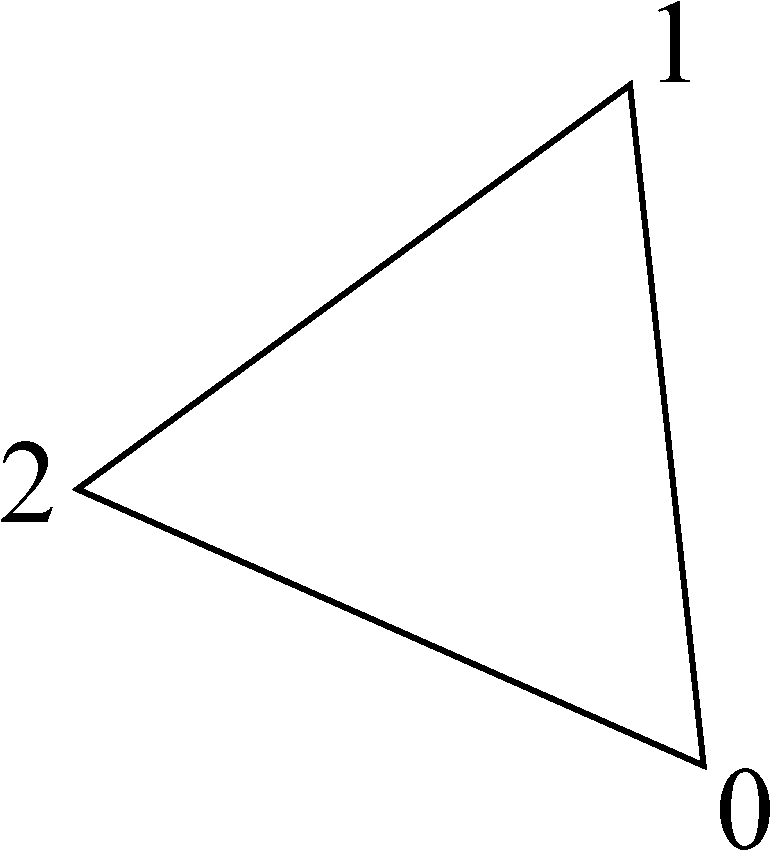
\includegraphics[width=1in]{s1.pdf}
   	\end{center}
\end{figure}
\FloatBarrier

To build a simplicial complex in javaPlex we simply build a stream in which all filtration times are zero. First we create an empty explicit simplex stream. Many command lines in this tutorial will end with a semicolon to supress unwanted output.

\begin{quote} \begin{verbatim} 
>> stream = api.Plex4.createExplicitSimplexStream();
\end{verbatim} \end{quote}

Next we add simplicies using the methods \texttt{addVertex} and \texttt{addElement}. The first creates a vertex with a specified index, and the second creates a $k$-simplex (for $k >0$) with the specified array of vertices. Since we don't specify any filtration times, by default all added simplices will have filtration time zero.

\begin{quote} \begin{verbatim}
>> stream.addVertex(0);
>> stream.addVertex(1);
>> stream.addVertex(2);
>> stream.addElement([0, 1]);
>> stream.addElement([0, 2]);
>> stream.addElement([1, 2]);
>> stream.finalizeStream();
\end{verbatim} \end{quote}

We print the total number of simplices in the complex.

\begin{quote} \begin{verbatim}
>> num_simplices = stream.getSize()
num_simplices = 6
\end{verbatim} \end{quote}

We create an object that will compute the homology of our complex. The first input parameter 3 indicates that homology will be computed in dimensions 0, 1, and 2 --- that is, in all dimensions strictly less than 3. The second input 2 means that we will compute homology with $\mathbb{Z}_2$ coefficients, and this input can be any prime number.

\begin{quote} \begin{verbatim}
>> persistence = api.Plex4.getModularSimplicialAlgorithm(3, 2);
\end{verbatim} \end{quote}

We compute and print the intervals.

\begin{quote} \begin{verbatim}
>> circle_intervals = persistence.computeIntervals(stream)
circle_intervals =

Dimension: 1
[0.0, infinity)
Dimension: 0
[0.0, infinity)
\end{verbatim} \end{quote}

This gives us the expected Betti numbers $Betti_0=1$ and $Betti_1=1$.

The persistence algorithm computing intervals can also find a representative cycle for each interval. However, there is no guarantee that the produced representative will be geometrically nice.

\begin{quote} \begin{verbatim}
>> circle_intervals = persistence.computeAnnotatedIntervals(stream)
circle_intervals =

Dimension: 1
[0.0, infinity): [1,2] + [0,2] + [0,1]
Dimension: 0
[0.0, infinity): [0]
\end{verbatim} \end{quote}

A representative cycle generating the single 0-dimensional homology class is [0], and a representative cycle generating the single 1-dimensional homology class is [1,2] + [0,2] + [0,1].

{\em 9-sphere example.} Let's build a 9-sphere, which is homeomorphic to the boundary of a 10-simplex. First we add a single 10-simplex to an empty explicit simplex stream. The result is not a simplicial complex because it does not contain the faces of the 10-simplex. We add all faces using the method \texttt{ensureAllFaces}. Then, we remove the 10-simplex using the method \texttt{removeElementIfPresent}. What remains is the boundary of a 10-simplex, that is, a 9-sphere.

\begin{quote} \begin{verbatim}
>> dimension = 9;
>> stream = api.Plex4.createExplicitSimplexStream();
>> stream.addElement(0:(dimension + 1));
>> stream.ensureAllFaces();
>> stream.removeElementIfPresent(0:(dimension + 1));
>> stream.finalizeStream();
\end{verbatim} \end{quote}

In the above, the \texttt{finalizeStream} function is used to ensure that the stream has been fully constructed and is ready for consumption by a persistence algorithm. Note that it can be omitted in the case where the simplex additions are done in increasing order. However, it should be used in general. 

We print the total number of simplices in the complex.

\begin{quote} \begin{verbatim}
>> num_simplices = stream.getSize()
num_simplices = 2046
\end{verbatim} \end{quote}

We get the persistence algorithm

\begin{quote} \begin{verbatim}
persistence = api.Plex4.getModularSimplicialAlgorithm(dimension + 1, 2);
\end{verbatim} \end{quote}

and compute and print the intervals.

\begin{quote} \begin{verbatim}
>> n_sphere_intervals = persistence.computeIntervals(stream)
n_sphere_intervals =

Dimension: 9
[0.0, infinity)
Dimension: 0
[0.0, infinity)
\end{verbatim} \end{quote}

This gives us the expected Betti numbers $Betti_0=1$ and $Betti_9=1$.

Try computing a representative cycle for each barcode.

\begin{quote} \begin{verbatim}
>> n_sphere_intervals = persistence.computeAnnotatedIntervals(stream)
\end{verbatim} \end{quote}

We don't display the output from this command in the tutorial, because the representative 9-cycle is very long and contains all eleven 9-simplices.

See Appendix \ref{A:solutions} for exercise solutions. 

\begin{exercise}
Build a simplicial complex homeomorphic to the torus. Compute its Betti numbers. {\em Hint: You will need at least 7 vertices} \citep[page 107]{Hatcher}{\em . We recommend using a $3\times 3$ grid of 9 vertices.} 
\end{exercise}

\begin{exercise}
Build a simplicial complex homeomorphic to the Klein bottle. Check that it has the same Betti numbers as the torus over $\mathbb{Z}_2$ coefficients but different Betti numbers over $\mathbb{Z}_3$ coefficients. 
\end{exercise}

\begin{exercise}
Build a simplicial complex homeomorphic to the projective plane. Find its Betti numbers over $\mathbb{Z}_2$ and $\mathbb{Z}_3$ coefficients. 
\end{exercise}


\subsection{Computing persistent homology}\label{computingPersistentHomology}

Let's build a stream with nontrivial filtration times. 

{\em House example.} The Matlab script corresponding to this section is \href{https://github.com/javaplex/javaplex/tree/master/src/matlab/for_distribution/tutorial_examples/house_example.m}{\texttt{house\_example.m}}.

\begin{wrapfigure}{r}{1in}
	\begin{center}
   	
\includegraphics[width=1in]{houseFig.pdf}
  	\end{center}
\end{wrapfigure}

We build a house, with the vertices and edges on the square appearing at time 0, with the top vertex appearing at time 1, with the roof edges appearing at times 2 and 3, and with the roof 2-simplex appearing at time 7.

\begin{quote} \begin{verbatim}
>> stream = api.Plex4.createExplicitSimplexStream();
>> stream.addVertex(1, 0);
>> stream.addVertex(2, 0);
>> stream.addVertex(3, 0);
>> stream.addVertex(4, 0);
>> stream.addVertex(5, 1);
>> stream.addElement([1, 2], 0);
>> stream.addElement([2, 3], 0);
>> stream.addElement([3, 4], 0);
>> stream.addElement([4, 1], 0);
>> stream.addElement([3, 5], 2);
>> stream.addElement([4, 5], 3);
>> stream.addElement([3, 4, 5], 7);
>> stream.finalizeStream();
\end{verbatim} \end{quote}

We get the persistence algorithm with $\mathbb{Z}_2$ coefficients
\begin{quote} \begin{verbatim}
>> persistence = api.Plex4.getModularSimplicialAlgorithm(3, 2);
\end{verbatim} \end{quote}

and compute the intervals.

\begin{quote} \begin{verbatim}
>> intervals = persistence.computeIntervals(stream)
intervals =

Dimension: 1
[3.0, 7.0)
[0.0, infinity)
Dimension: 0
[1.0, 2.0)
[0.0, infinity)
\end{verbatim} \end{quote}

There are four intervals. The first is a $Betti_1$ interval, starting at filtration time 3 and ending at 7. This 1-dimensional hole is formed by the three edges of the roof. It forms when edge $[4,5]$ appears at filtration time 3 and closes when 2-simplex $[3,4,5]$ appears at filtration time 7.

We can also store the intervals as Matlab matrices.

\begin{quote} \begin{verbatim}
>> intervals_dim0 = edu.stanford.math.plex4.homology.barcodes.BarcodeUtility...
.getEndpoints(intervals, 0, 0)
intervals_dim0 =

    0    Inf
    1    2
    
>> intervals_dim1 = edu.stanford.math.plex4.homology.barcodes.BarcodeUtility...
.getEndpoints(intervals, 1, 0)
intervals_dim1 =

    0    Inf
    3    7
\end{verbatim} \end{quote}

The second input of this command is the dimension of the intervals, and the third input is a Boolean flag: 0 to include infinite intervals, and 1 to exclude infinite intervals.

We compute a representative cycle for each barcode.

\begin{quote} \begin{verbatim}
>> intervals = persistence.computeAnnotatedIntervals(stream)
intervals =

Dimension: 1
[3.0, 7.0): [4,5] + [3,4] + -[3,5]
[0.0, infinity): [1,4] + [2,3] + [1,2] + [3,4]
Dimension: 0
[1.0, 2.0): -[3] + [5]
[0.0, infinity): [1]
\end{verbatim} \end{quote}

One $Betti_0$ interval and one $Betti_1$ interval are semi-infinite. 
\begin{quote} \begin{verbatim}
>> infinite_barcodes = intervals.getInfiniteIntervals();
\end{verbatim} \end{quote}

We can print the Betti numbers (at the largest filtration time 7) as an array

\begin{quote} \begin{verbatim}
>> betti_numbers_array = infinite_barcodes.getBettiSequence()
betti_numbers_array =

    1
    1
\end{verbatim} \end{quote}

or as a list with entries of the form $k: Betti_k$.

\begin{quote} \begin{verbatim}
>> betti_numbers_string = infinite_barcodes.getBettiNumbers()
betti_numbers_string = {0: 1, 1: 1} 
\end{verbatim} \end{quote}

The Matlab function \texttt{plot\_barcodes.m} lets us display the intervals as Betti barcodes. The Matlab structure array \texttt{options} contains different options for the plot. We choose the filename \texttt{house} and we choose the maximum filtration time for the plot to be eight.
\begin{quote} \begin{verbatim}
>> options.filename = 'house';
>> options.max_filtration_value = 8;
>> plot_barcodes(intervals, options);
\end{verbatim} \end{quote}

The file \texttt{house.png} is saved to your current directory.

\begin{figure}[htp]
	\begin{center}
    	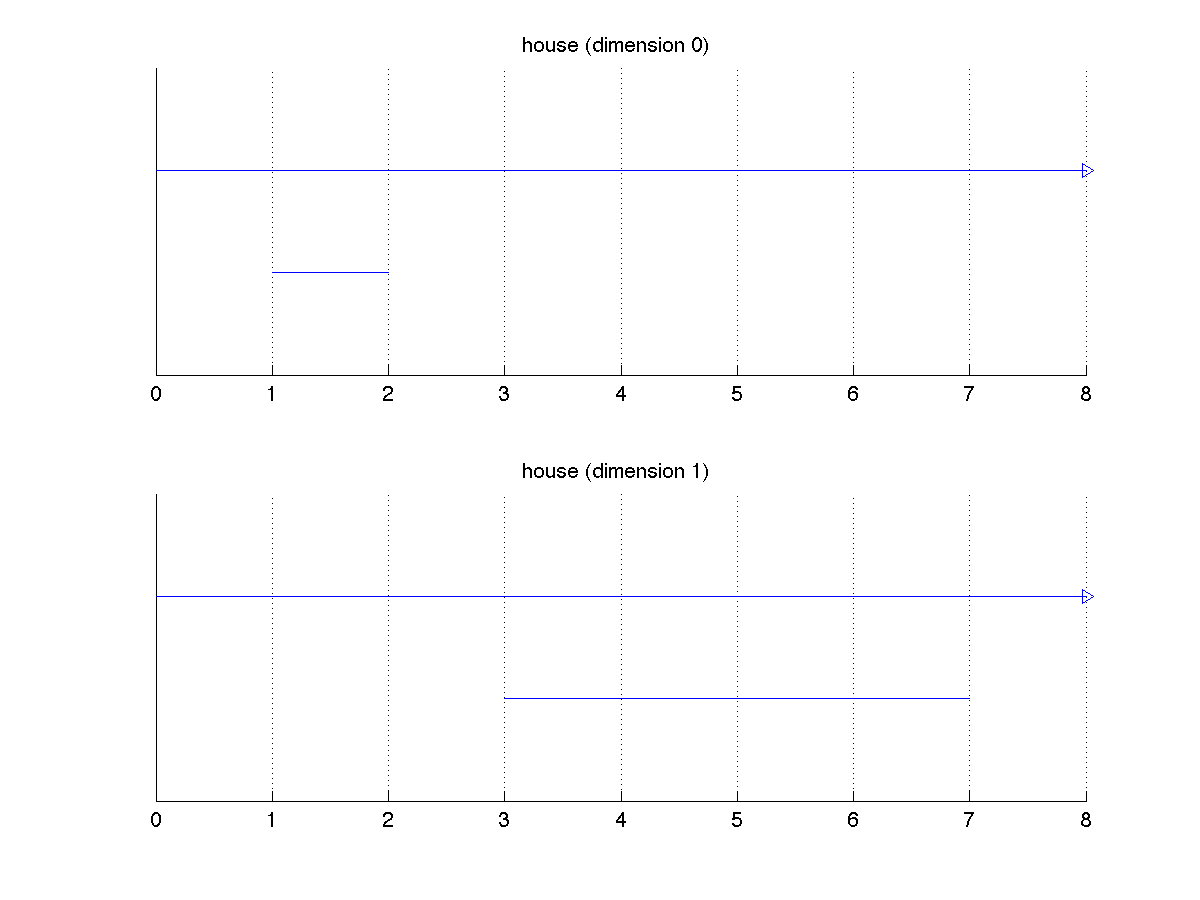
\includegraphics[width=6in]{house.png}
   	\end{center}
\end{figure}
\FloatBarrier

The filtration times are on the horizontal axis. The $Betti_k$ number of the stream at filtration time $t$ is the number of intervals in the dimension $k$ plot that intersect a vertical line through $t$. Check that the displayed intervals agree with the filtration times we built into the house stream. At time 0, a connected component and a 1-dimensional hole form. At time 1, a second connected component appears, which joins to the first at time 2. A second 1-dimensional hole forms at time 3, and closes at time 7. 

{\em Remark.} The methods \texttt{addElement} and \texttt{removeElementIfPresent} do not necessarily enforce the definition of a stream. They allow us to build inconsistent complexes in which some simplex $\sigma \in X(t)$ contains a subsimplex $\sigma' \notin X(t)$, meaning that $X(t)$ is not a simplicial complex. The method \texttt{validateVerbose} returns \texttt{1} if our stream is consistent and returns \texttt{0} with explanation if not. 

\begin{quote} \begin{verbatim}
>> stream.validateVerbose()
ans = 1
>> stream.addElement([1, 4, 5], 0);
>> stream.validateVerbose()
Filtration index of face [4,5] exceeds that of element [1,4,5] (3 > 0)
Stream does not contain face [1,5] of element [1,4,5]
ans = 0
\end{verbatim} \end{quote}

{\em Remark.} If you want to use filtration times that are not integers, then you first need to specify an upper bound on the filtration times in your complex. This is demonstrated below, where the non-integer filtration time is 17.23 and the upper bound is 100.

\begin{quote} \begin{verbatim}
>> stream = api.Plex4.createExplicitSimplexStream(100);
>> stream.addVertex(1, 17.23);
>> stream.finalizeStream();
\end{verbatim} \end{quote}

%In Section \ref{sfpc} we will create simplex streams that are not also explicit simplex streams. To display or edit such streams, we will first need to use the method \texttt{makeExplicit}. See Exercise \ref{ripsExpl}. 

% Henry: At the moment there is no ``make Explicit'' function. 




\section{Point cloud data}

A point cloud is a finite metric space, that is, a finite set of points equipped with a notion of distance. One can create a Euclidean metric space by specifying the coordinates of points in Euclidean space, or one can create an explicit metric space by specifying all pairwise distances between points. In Section \ref{sfpc} we will learn how to build streams from point cloud data. 


\subsection{Euclidean metric spaces}\label{euc} The Matlab script corresponding to this section is \href{https://github.com/javaplex/javaplex/tree/master/src/matlab/for_distribution/tutorial_examples/pointcloud_example.m}{\texttt{pointcloud\_example.m}}. 

{\em House example.} Let's give Euclidean coordinates to the points of our house.

\vspace{-3mm}
\begin{figure}[htb]
	\centering
	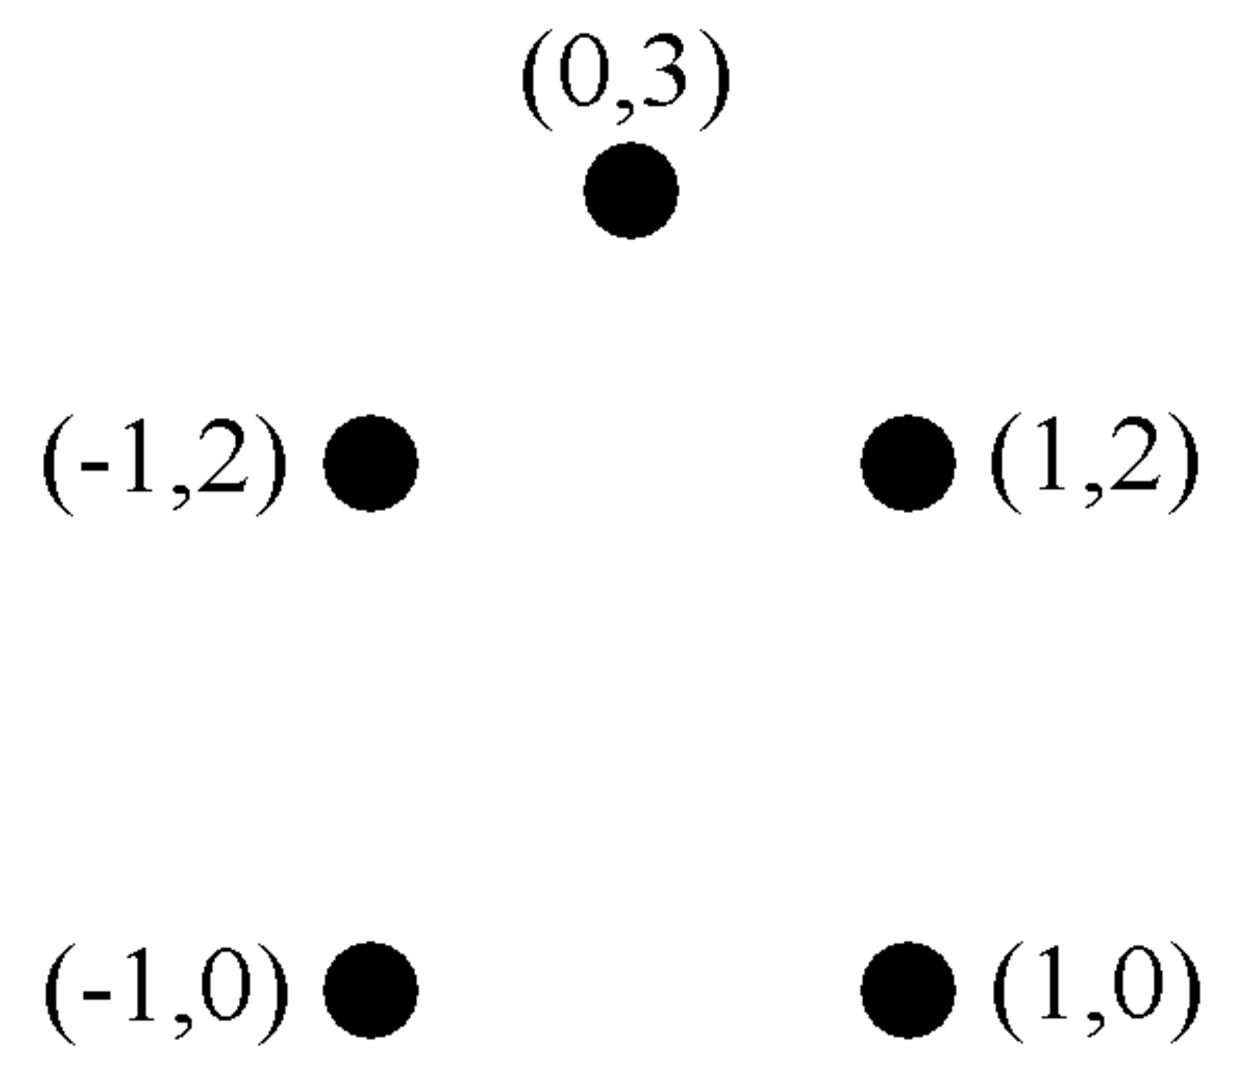
\includegraphics[width=1.55in]{houseCoord.pdf}
	\vspace{-3mm}
	\caption{The house point cloud}
	\label{fig:housePointCloud}
\end{figure}
\FloatBarrier

You can enter these coordinates manually.

\begin{quote} \begin{verbatim}
>> point_cloud = [-1,0; 1,0; 1,2; -1,2; 0,3]
point_cloud =

   -1    0
    1    0
    1    2
   -1    2
    0    3
\end{verbatim} \end{quote}

Or, these coordinates are stored as a javaPlex example.

\begin{quote} \begin{verbatim}
>> point_cloud = examples.PointCloudExamples.getHouseExample();
\end{verbatim} \end{quote}

We create a metric space using these coordinates. The input to the \texttt{EuclideanMetricSpace} method is a matrix whose $i$-th row lists the coordinates of the $i$-th point.

\begin{quote} \begin{verbatim}
>> m_space = metric.impl.EuclideanMetricSpace(point_cloud); 
\end{verbatim} \end{quote}

We can return the coordinates of a specific point. Note the points are indexed starting at 0.

\begin{quote} \begin{verbatim}
>> m_space.getPoint(0)
ans = 

   -1
    0
   
>> m_space.getPoint(2)
ans = 

    1
    2
\end{verbatim} \end{quote}

A metric space can return the distance between any two points.

\begin{quote} \begin{verbatim}
>> m_space.distance(m_space.getPoint(0), m_space.getPoint(2))
ans = 2.8284
\end{verbatim} \end{quote}

{\em Figure 8 example.} We select 1,000 points randomly from a figure eight, that is, the union of unit circles centered at $(0,1)$ and $(0,-1)$.

\begin{quote} \begin{verbatim}
>> point_cloud = examples.PointCloudExamples.getRandomFigure8Points(1000);
\end{verbatim} \end{quote}

We plot the points.

\begin{quote} \begin{verbatim}
>> figure
>> scatter(point_cloud(:,1), point_cloud(:,2), '.')
>> axis equal
\end{verbatim} \end{quote}

{\em Torus example.} We select 2,000 points randomly from a torus in $\mathbb{R}^3$ with inner radius 1 and outer radius 2. The first input is the number of points, the second input is the inner radius, and the third input is the outer radius

\begin{quote} \begin{verbatim}
>> point_cloud = examples.PointCloudExamples.getRandomTorusPoints(2000, 1, 2);
\end{verbatim} \end{quote}

We plot the points.

\begin{quote} \begin{verbatim}
>> figure
>> scatter3(point_cloud(:,1), point_cloud(:,2), point_cloud(:,3), '.')
>> axis equal
\end{verbatim} \end{quote}

{\em Sphere product example.} We select 1,000 points randomly from the unit torus $S^1 \times S^1$ in $\mathbb{R}^4$. The first input is the number of points, the second input is the dimension of each sphere, and the third input is the number of sphere factors.

\begin{quote} \begin{verbatim}
>> point_cloud = examples.PointCloudExamples.getRandomSphereProductPoints(1000, 1, 2);
\end{verbatim} \end{quote}

Plotting the third and fourth coordinates of each point shows a circle $S^1$.

\begin{quote} \begin{verbatim}
>> figure
>> scatter(point_cloud(:,3), point_cloud(:,4), '.')
>> axis equal
\end{verbatim} \end{quote}


\subsection{Explicit metric spaces}
We can also create a metric space from a distance matrix using the method \texttt{ExplicitMetricSpace}. For a point cloud in Euclidean space, this method is generally less convenient than the command \texttt{EuclideanMetricSpace}. However, method \texttt{ExplicitMetricSpace} can be used for a point cloud in an arbitrary (perhaps non-Euclidean) metric space. 

The Matlab script corresponding to this section is \href{https://github.com/javaplex/javaplex/tree/master/src/matlab/for_distribution/tutorial_examples/explicit_metric_space_example.m}{\texttt{explicit\_metric\_space\_example.m}}. 

{\em House example.} The matrix \texttt{distances} summarizes the metric for our house points in Figure \ref{fig:housePointCloud}: entry $(i,j)$ is the distance from point $i$ to point $j$. 

\begin{quote} \begin{verbatim}
>> distances = [0,2,sqrt(8),2,sqrt(10);
2,0,2,sqrt(8),sqrt(10);
sqrt(8),2,0,2,sqrt(2);
2,sqrt(8),2,0,sqrt(2);
sqrt(10),sqrt(10),sqrt(2),sqrt(2),0]

distances =

    0         2.0000    2.8284    2.0000    3.1623
    2.0000    0         2.0000    2.8284    3.1623
    2.8284    2.0000    0         2.0000    1.4142
    2.0000    2.8482    2.0000    0         1.4142
    3.1623    3.1623    1.4142    1.4142    0
\end{verbatim} \end{quote}

We create a metric space from this distance matrix.

\begin{quote} \begin{verbatim}
>> m_space = metric.impl.ExplicitMetricSpace(distances);
\end{verbatim} \end{quote}

We return the distance between points 0 and 2.

\begin{quote} \begin{verbatim}
>> m_space.distance(0, 2)
ans = 2.8284 
\end{verbatim} \end{quote}

% Be careful: the constructor \texttt{DistanceData()} will accept matrices that fail to be symmetric, square, or nonnegative, creating ``metrics'' that do not satisfy the mathematical definiton. The triangle inequality is similarly easy to ignore. However, asking for the distance between a point and itself will always return zero, even if you input a distance matrix with non-zero diagonal entries. 

\begin{exercise}\label{Ex:flatTorus}
One way to produce a torus is to take a square $[0, 1] \times [0, 1]$ and then identify opposite sides. This is called a flat torus. More explicitly, the quotient space
$$([0, 1] \times [0, 1]) / \sim,$$
where $(0, y) \sim (1, y)$ for all $y \in [0, 1]$ and where $(x, 0) \sim (x, 1)$ for all $x \in [0, 1]$, is a flat torus. The Euclidean metric on $[0, 1] \times [0, 1]$ induces a metric on the flat torus. For example, in the induced metric on the flat torus, the distance between $(0, \frac{1}{2})$ and $(1, \frac{1}{2})$ is zero, since these two points are identified. The distance between $(\frac{1}{10}, \frac{1}{2})$ and $(\frac{9}{10}, \frac{1}{2})$ is $\frac{2}{10}$, by passing through the point $(0, \frac{1}{2}) \sim (1, \frac{1}{2})$.

Write a Matlab script or function that selects 1,000 random points from the square $[0, 1] \times [0, 1]$ and then computes the 1,000 $\times$ 1,000 distance matrix for these points under the induced metric on the flat torus. Create an explicit metric space from this distance matrix. 

This exercise is continued by Exercise \ref{Ex:flatTorusLazy}. 

% TODO: Gard Spreeman at MRC gave me a good idea for the Matlab function FlatTorusDistanceMatrix.m: just move one point to the center of the square, and then find the distance in the square to the other point.
\end{exercise}

\begin{exercise}\label{Ex:flatKlein}
One way to produce a Klein bottle is to take a square $[0, 1] \times [0, 1]$ and then identify opposite edges, with the left and right sides identified with a twist. This is called a flat Klein bottle. More explicitly, the quotient space 
$$([0, 1] \times [0, 1]) / \sim,$$
where $(0, y) \sim (1, 1 - y)$ for all $y \in [0, 1]$ and where $(x, 0) \sim (x, 1)$ for all $x \in [0, 1]$, is a flat Klein bottle. The Euclidean metric on $[0, 1] \times [0, 1]$ induces a metric on the flat Klein bottle. For example, in the induced metric on the flat Klein bottle, the distance between $(0, \frac{4}{10})$ and $(1, \frac{6}{10})$ is zero, since these two points are identified. The distance between $(\frac{1}{10}, \frac{4}{10})$ and $(\frac{9}{10}, \frac{6}{10})$ is $\frac{2}{10}$, by passing through the point $(0, \frac{4}{10}) \sim (1, \frac{6}{10})$.

Write a Matlab script or function that selects 1,000 random points from the square $[0, 1] \times [0, 1]$ and then computes the 1,000 $\times$ 1,000 distance matrix for these points under the induced metric on the flat Klein bottle. Create an explicit metric space from this distance matrix. 

This exercise is continued by Exercise \ref{Ex:flatKleinLazy}. 
\end{exercise}

\begin{exercise}\label{Ex:quotProjPlane}
One way to produce a projective plane is to take the unit sphere $S^2 \subset \mathbb{R}^3$ and then identify antipodal points. More explicitly, the quotient space 
$$S^2 / (x \sim -x)$$
is a projective plane. The Euclidean metric on $S^2$ induces a metric on the projective plane.

Write a Matlab script or function that selects 1,000 random points from the unit sphere $S^2 \subset \mathbb{R}^3$ and then computes the 1,000 $\times$ 1,000 distance matrix for these points under the induced metric on the projective plane. Create an explicit metric space from this distance matrix. 

This exercise is continued by Exercise \ref{Ex:quotProjPlaneLazy}. 
\end{exercise}




\section{Streams from point cloud data}\label{sfpc}

In Section \ref{explicitStream} we built streams explicitly, or by hand. In this section we construct streams from a point cloud $Z$. We build Vietoris--Rips, witness, and lazy witness streams. See \citet{WitnessComplexes} for additional information. 

The Vietoris--Rips, witness, and lazy witness streams all take three of the same inputs: the maximum dimension $d_{max}$, the maximum filtration time $t_{max}$, and the number of divisions $N$. These inputs allow the user to limit the size of the constructed stream, for computational efficiency. No simplices above dimension $d_{max}$ are included. The persistent homology of the resulting stream can be calculated only up to dimension $d_{max} - 1$ (do you see why?). Also, instead of computing complex $X(t)$ for all $t \geq 0$, we only compute $X(t)$ for
$$t \in \Biggl\{ 0,\ \frac{t_{max}}{N-1},\ \frac{2t_{max}}{N-1},\ \frac{3t_{max}}{N-1},\ \dots,\ \frac{(N-2)t_{max}}{N-1},\ t_{max} \Biggr\}.$$
The number of divisions $N$ is an optional input. If this input parameter is not specified, then the default value $N = 20$ is used. 

When working with a new dataset, don't choose $d_{max}$ and $t_{max}$ too large initially. First get a feel for how fast the simplicial complexes are growing, and then raise $d_{max}$ and $t_{max}$ nearer to the computational limits. If you ever choose $d_{max}$ or $t_{max}$ too large and Matlab seems to be running forever, pressing the \texttt{control} and \texttt{c} buttons simultaneously may halt the computation. 

%The first author is currently working with Jan Segert on interactive visualizations of the Vietoris--Rips and Witness filtrations for the Wolfram Demonstrations Project. We have preliminary drafts of the demonstrations. Please email Henry if you'd like to check them out; in particular, the witness filtrations can be hard to visualize. 


\subsection{Vietoris--Rips streams}\label{Vietoris--Rips}
Let  $d(\ \cdot\ ,\ \cdot \ )$ denote the distance between two points in metric space $Z$. A natural stream to build is the Vietoris--Rips stream. The complex $\VR(Z,t)$ is defined as follows: 
\begin{itemize}
\item{the vertex set is $Z$.}
\item{for vertices $a$ and $b$, edge $[ab]$ is in $\VR(Z,t)$ if $d(a,b) \leq t$.}
\item{a higher dimensional simplex is in $\VR(Z,t)$ if all of its edges are.}
\end{itemize}
Note that $\VR(Z,t) \subset \VR(Z,s)$ whenever $t\leq s$, so the Vietoris--Rips stream is a filtered simplicial complex. Since a Vietoris--Rips complex is the maximal simplicial complex that can be built on top of its 1-skeleton, it is a {\em flag complex}. 

The Matlab script corresponding to this section is \href{https://github.com/javaplex/javaplex/tree/master/src/matlab/for_distribution/tutorial_examples/rips_example.m}{\texttt{rips\_example.m}}. 

{\em House example.} Let's build a Vietoris--Rips stream from the house point cloud in Section \ref{euc}. Note this stream is different than the explicit house stream we built in Section \ref{computingPersistentHomology}.

\begin{quote} \begin{verbatim}
>> max_dimension = 3;
>> max_filtration_value = 4;
>> num_divisions = 100;

>> point_cloud = examples.PointCloudExamples.getHouseExample();
>> stream = api.Plex4.createVietorisRipsStream(point_cloud, max_dimension, ...
max_filtration_value, num_divisions);
\end{verbatim} \end{quote}

The ellipses in the command above should be omitted; they are included only to indicate that this command continues onto the next line. 

The order of the inputs is \texttt{createVietorisRipsStream(}$Z,\ d_{max},\ t_{max},\ N$\texttt{)}. For a Vietoris--Rips stream, the parameter $t_{max}$ is the maximum possible edge length. Since $t_{max} = 4$ is greater than the diameter ($\sqrt{10}$) of our point cloud, all edges will eventually form. 

Since $d_{max} = 3$ we can compute up to second dimensional persistent homology.

\begin{quote} \begin{verbatim}
>> persistence = api.Plex4.getModularSimplicialAlgorithm(max_dimension, 2);
>> intervals = persistence.computeIntervals(stream);
\end{verbatim} \end{quote}

We display the Betti intervals. Parameter \texttt{options.max\_filtration\_value} is the largest filtration time to be displayed. Typically \texttt{options.max\_filtration\_value} is chosen to be \texttt{max\_filtration\_value}. Parameter \texttt{options.max\_dimension} is the largest persistent homology dimension to be displayed. Typically \texttt{options.max\_dimension} is chosen to be \texttt{max\_dimension - 1} because in a stream with simplices computed up to dimension $d_{max}$ we can only compute persistent homology up to dimension $d_{max} - 1$.

\begin{quote} \begin{verbatim}
>> options.filename = 'ripsHouse';
>> options.max_filtration_value = max_filtration_value;
>> options.max_dimension = max_dimension - 1;
>> plot_barcodes(intervals, options);
\end{verbatim} \end{quote}

The file \texttt{ripsHouse.png} is saved to your current directory.

\begin{figure}[htp]
	\begin{center}
    	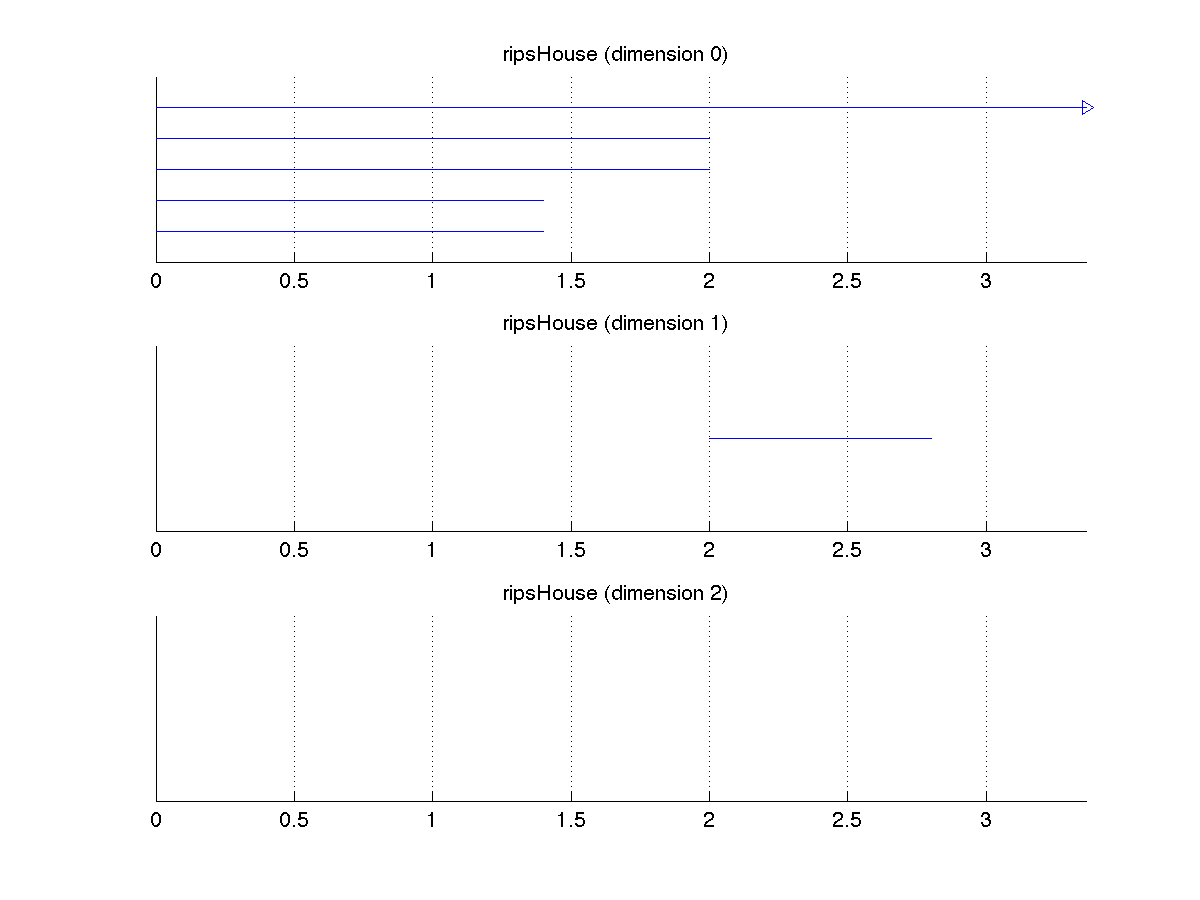
\includegraphics[width=6in]{ripsHouse.png}
   	\end{center}
\end{figure}
\FloatBarrier

Check that these plots are consistent with the Vietoris--Rips definition: edges $[3,5]$ and $[4,5]$ appear at filtration time $t = \sqrt{2}$; the square appears at $t = 2$; the square closes at $t = \sqrt{8}$. 

%\begin{exercise}
%Change \texttt{ripsHouse} into an explicit stream
%
%\begin{quote} \begin{verbatim}
%>> ripsExpl = Plex.makeExplicit(ripsHouse);
%\end{verbatim} \end{quote} 
%
%Check that you can display and edit stream \texttt{ripsExpl} using the methods of Section \ref{explicitStream}. 
%\end{exercise}

% Is the above exercise no longer necessary, or no longer possible?
% Answer: At the moment it isn't possible. Do you think it is meaningful?

% Is there a way to print the simplices in a stream (and perhaps their filtration times?

{\em Torus example.} Try the following sequence of commands. We start with 400 points from a $20 \times 20$ grid on the unit torus $S^1 \times S^1$ in $\mathbb{R}^4$, and add a small amount of noise to each point.
% If I select points randomly from the torus instead from the regular grid, then the Vietoris--Rips stream does not seem to be able to recover the correct Betti numbers.
We build the Vietoris--Rips stream.

\begin{quote} \begin{verbatim}
>> max_dimension = 3;
>> max_filtration_value = 0.9;
>> num_divisions = 100;
\end{verbatim} \end{quote}

Load the file \href{https://github.com/javaplex/javaplex/tree/master/src/matlab/for_distribution/tutorial_examples/pointsTorusGrid.mat}{\texttt{pointsTorusGrid.mat}}. The matrix \texttt{pointsTorusGrid} appears in your Matlab workspace.

\begin{quote} \begin{verbatim}
>> load pointsTorusGrid.mat
>> point_cloud = pointsTorusGrid;
>> size(point_cloud)
ans = 400    4                         % 400 points in dimension 4

>> stream = api.Plex4.createVietorisRipsStream(point_cloud, max_dimension, ...
max_filtration_value, num_divisions); 
>> num_simplices = stream.getSize()
num_simplices = 82479

>> persistence = api.Plex4.getModularSimplicialAlgorithm(max_dimension, 2);
>> intervals = persistence.computeIntervals(stream);

>> options.filename = 'ripsTorus';
>> options.max_filtration_value = max_filtration_value;
>> options.max_dimension = max_dimension - 1;
>> options.side_by_side = true;
>> plot_barcodes(intervals, options);
\end{verbatim} \end{quote}

Setting the parameter \texttt{options.side\_by\_side} equal to \texttt{true} makes it such that the Betti barcodes of different dimensions are plotted side by side instead of above and below each other. The file \texttt{ripsTorus.png} is saved to your current directory.

\begin{figure}[htp]
	\begin{center}
    	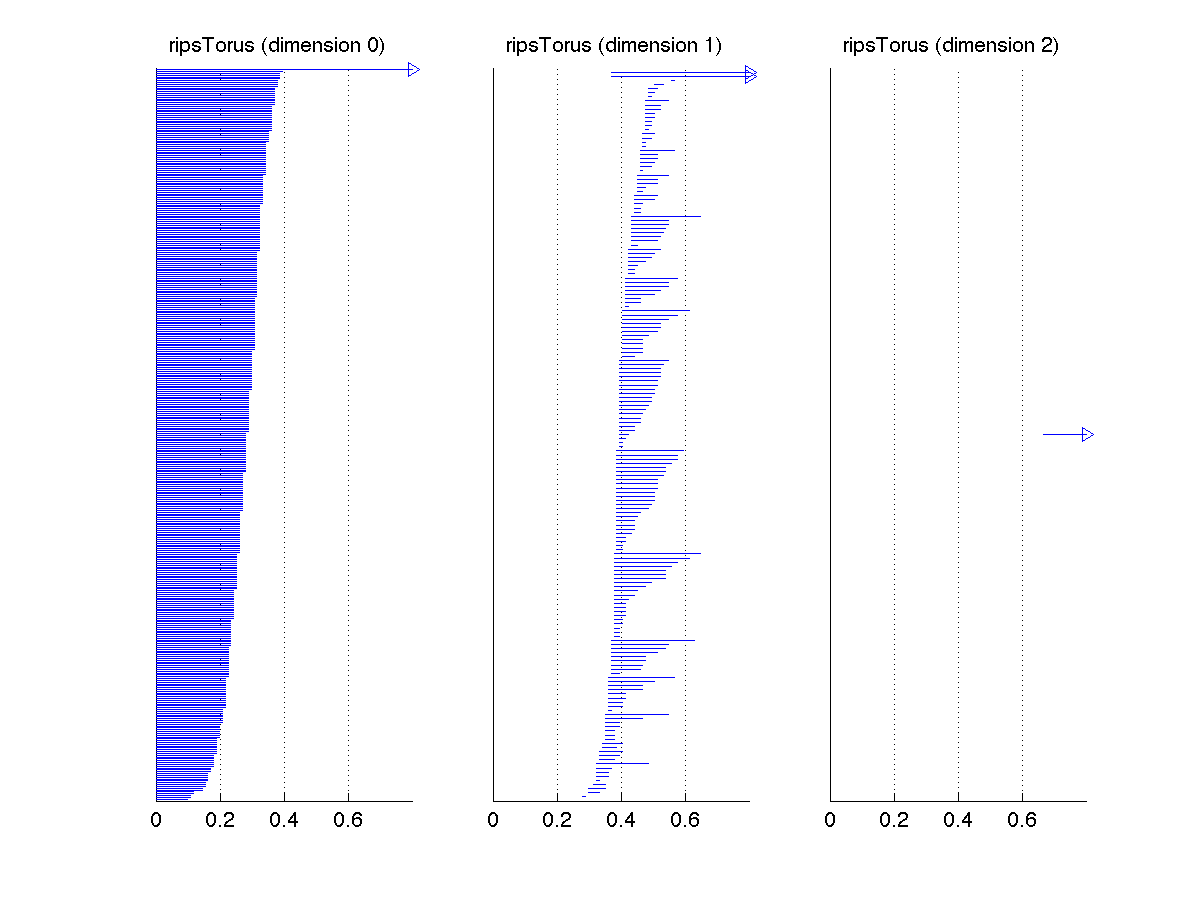
\includegraphics[width=6in]{ripsTorus.png}
   	\end{center}
\end{figure}
\FloatBarrier

The diameter of this torus (before adding noise) is $\sqrt{8}$, so choosing $t_{max} = 0.9$ likely will not show all homological activity. However, the torus will be reasonably connected by this time. Note the semi-infinite intervals match the correct numbers $Betti_0 = 1$, $Betti_1 = 2$, $Betti_2 = 1$ for a torus.

\begin{quote} \begin{verbatim}
>> infinite_barcodes = intervals.getInfiniteIntervals();
>> betti_numbers_array = infinite_barcodes.getBettiSequence()
betti_numbers_array =

    1
    2
    1
\end{verbatim} \end{quote}

This example makes it clear that the computed ``semi-infinite'' intervals do not necessarily persist until $t = \infty$: in a Vietoris--Rips stream, once $t$ is greater than the diameter of the point cloud, the Betti numbers for $\VR(Z,t)$ will be $ Betti_0 = 1$, $Betti_1 = Betti_2 = ... = 0$. The computed semi-infinite intervals are merely those that persist until $t = t_{max}$. 

{\em Remark.} We can build Vietoris--Rips streams not only on top of Euclidean point clouds, but also on top of explicit metric spaces. For example, if \texttt{m\_space} were an explicit metric space, then we could call a command such as

\begin{quote} \begin{verbatim}
>> stream = api.Plex4.createVietorisRipsStream(m_space, max_dimension, ...
max_filtration_value, num_divisions);  
\end{verbatim} \end{quote}

\begin{exercise}
Slowly increase the values for $t_{max}$, $d_{max}$ and note how quickly the size of the Vietoris--Rips stream and the time of computation grow. Either increasing $t_{max}$ from 0.9 to 1 or increasing $d_{max}$ from 3 to 4 roughly doubles the size of the Vietoris--Rips stream. 
\end{exercise}

\begin{exercise}
Find a planar dataset $Z \subset \mathbb{R}^2$ and a filtration value $t$ such that $\VR(Z,t)$ has nonzero $Betti_2$. Build a Vietoris--Rips stream to confirm your answer. 
\end{exercise}

\begin{exercise}
Find a planar dataset $Z \subset \mathbb{R}^2$ and a filtration value $t$ such that $\VR(Z,t)$ has nonzero $Betti_6$. When building a Vietoris--Rips stream to confirm your answer, don't forget to choose $d_{max} = 7$. 
\end{exercise}


\subsection{Landmark selection}\label{lands}
For larger datasets, if we include every data point as a vertex, as in the Vietoris--Rips construction, our streams will quickly contain too many simplices for efficient computation. The witness stream and the lazy witness stream address this problem. In building these streams, we select a subset $L \subset Z$, called landmark points, as the only vertices. All data points in $Z$ help serve as witnesses for the inclusion of higher dimensional simplices. 

There are two common methods for selecting landmark points. The first is to choose the landmarks $L$ randomly from point cloud $Z$. The second is a greedy inductive selection process called sequential maxmin. In sequential maxmin, the first landmark is picked randomly from $Z$. Inductively, if $L_{i-1}$ is the set of the first $i-1$ landmarks, then let the $i$-th landmark be the point of $Z$ which maximizes the function $z \mapsto d(z, L_{i-1})$, where $d(z, L_{i-1})$ is the distance between the point $z$ and the set $L_{i-1}$. 

Landmarks chosen using sequential maxmin tend to cover the dataset and to be spread apart from each other. A disadvantage is that outlier points tend to be selected. However, outlier points are less of an issue if one first takes dense core subsets as in Appendix \ref{A:core}. Sequential maxmin landmarks are used by \citet{Range} and \citet{KleinBottle}. 

The Matlab script corresponding to this section is \href{https://github.com/javaplex/javaplex/tree/master/src/matlab/for_distribution/tutorial_examples/landmark_example.m}{\texttt{landmark\_example.m}}.

{\em Figure 8 example.} We create a point cloud of 1,000 points from a figure eight.

\begin{quote} \begin{verbatim}
>> point_cloud = examples.PointCloudExamples.getRandomFigure8Points(1000);
\end{verbatim} \end{quote}

We create both a random landmark selector and a sequential maxmin landmark selector. These selectors will pick 100 landmarks each.

\begin{quote} \begin{verbatim}
>> num_landmark_points = 100;
>> random_selector = api.Plex4.createRandomSelector(point_cloud, num_landmark_points);
>> maxmin_selector = api.Plex4.createMaxMinSelector(point_cloud, num_landmark_points);
\end{verbatim} \end{quote}

We select 100 random landmarks and 100 landmarks via sequential maxmin. Note we need to increment the indices by 1 since Java uses 0-based arrays.

\begin{quote} \begin{verbatim}
>> random_points = point_cloud(random_selector.getLandmarkPoints() + 1, :);
>> maxmin_points = point_cloud(maxmin_selector.getLandmarkPoints() + 1, :);
\end{verbatim} \end{quote}

We plot the two sets of landmark points to see the difference between random and sequential maxmin landmark selection.

\begin{quote} \begin{verbatim}
>> subplot(1, 2, 1);
>> scatter(random_points(:,1), random_points(:, 2));
>> title('Random landmark selection');
>> subplot(1, 2, 2);
>> scatter(maxmin_points(:,1), maxmin_points(:, 2));
>> title('Maxmin landmark selection');
\end{verbatim} \end{quote}

\begin{figure}[htp]
  	\begin{center}
    	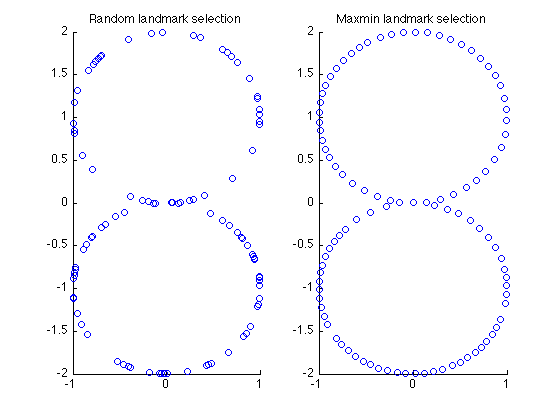
\includegraphics[width=5in]{fig8lands}
   	\end{center}
\end{figure}
\FloatBarrier

Sequential maxmin seems to do a better job of choosing landmarks that cover the figure eight and that are spread apart. 

{\em Remark.} We can select landmark points not only from Euclidean point clouds but also from explicit metric spaces. For example, if \texttt{m\_space} is an explicit metric space, then we may select landmarks using a command such as the following.

\begin{quote} \begin{verbatim}
>> maxmin_selector = api.Plex4.createMaxMinSelector(m_space, num_landmark_points); 
\end{verbatim} \end{quote}

Given point cloud $Z$ and landmark subset $L$, we define $\texttt{R} = \max_{z\in Z}\bigl\{d(z,L)\bigr\}$. Number \texttt{R} reflects how finely the landmarks cover the dataset. We often use it as a guide for selecting the maximum filtration value $t_{max}$ for a witness or lazy witness stream. 

\begin{exercise}
Let $Z$ be the point cloud in Figure \ref{fig:housePointCloud} from Section \ref{euc}, corresponding to the house point cloud. Suppose we are using sequential maxmin to select a set $L$ of 3 landmarks, and the first (randomly selected) landmark is $(1,0)$. Find by hand the other two landmarks in $L$. 
\end{exercise}

\begin{exercise}
Let $Z$ be a point cloud and $L$ a landmark subset. Show that if $L$ is chosen via sequential maxmin, then for any $l_i,l_j\in L$, we have $d(l_i,l_j)\geq\texttt{R}$. 
\end{exercise}


\subsection{Witness streams}
Suppose we are given a point cloud $Z$ and landmark subset $L$. Let $m_k(z)$ be the distance from a point $z \in Z$ to its $(k+1)$-th closest landmark point. The witness stream complex $\W(Z,L,t)$ is defined as follows.
\begin{itemize}
\item{the vertex set is $L$.}
\item{for $k>0$ and vertices $l_i$, the $k$-simplex $[l_0 l_1 ... l_k]$ is in $\W(Z,L,t)$ if all of its faces are, and if there exists a witness point $z \in Z$ such that $$\max\bigl\{d(l_0,z), d(l_1,z), ..., d(l_k,z)\bigr\} \leq t+m_k(z).$$ }
\end{itemize}
Note that $\W(Z,L,t) \subset \W(Z,L,s)$ whenever $t\leq s$. Note that a landmark point can serve as a witness point. 

\begin{exercise}\label{Ex:witnessHouse}
Let $Z$ be the point cloud in Figure \ref{fig:housePointCloud} from Section \ref{euc}, corresponding to the house point cloud. Let $L = \{(1,0),(0,3),(-1,0)\}$ be the landmark subset. Find by hand the filtration time for the edge between vertices $(1,0)$ and $(0,3)$. Which point or points witness this edge? What is the filtration time for the lone 2-simplex $[(1,0),(0,3),(-1,0)]$? 
\end{exercise}

The Matlab script corresponding to this section is \href{https://github.com/javaplex/javaplex/tree/master/src/matlab/for_distribution/tutorial_examples/witness_example.m}{\texttt{witness\_example.m}}.

{\em Torus example.} Let's build a witness stream instance for 10,000 random points from the unit torus $S^1 \times S^1$ in $\mathbb{R}^4$, with 50 sequential maxmin landmarks.

\begin{quote} \begin{verbatim}
>> num_points = 10000;
>> num_landmark_points = 50;
>> max_dimension = 3;
>> num_divisions = 100;

>> point_cloud = examples.PointCloudExamples.getRandomSphereProductPoints(num_points, ...
1, 2);
>> landmark_selector = api.Plex4.createMaxMinSelector(point_cloud, num_landmark_points);
\end{verbatim} \end{quote}

The next command returns the landmark covering measure \texttt{R} from Section \ref{lands}.  Often the value for $t_{max}$ is chosen in proportion to \texttt{R}.

\begin{quote} \begin{verbatim}
>> R = landmark_selector.getMaxDistanceFromPointsToLandmarks()
R = 0.7033                         % Generally close to 0.7
>> max_filtration_value = R / 8; 
\end{verbatim} \end{quote}

We create the witness stream.

\begin{quote} \begin{verbatim}
>> stream = api.Plex4.createWitnessStream(landmark_selector, max_dimension, ...
max_filtration_value, num_divisions); 
>> num_simplices = stream.getSize()
num_simplices = 1164                         % Generally close to 1200
\end{verbatim} \end{quote}

We plot the Betti intervals.

\begin{quote} \begin{verbatim}
>> persistence = api.Plex4.getModularSimplicialAlgorithm(max_dimension, 2);
>> intervals = persistence.computeIntervals(stream);

>> options.filename = 'witnessTorus';
>> options.max_filtration_value = max_filtration_value;
>> options.max_dimension = max_dimension - 1;
>> plot_barcodes(intervals, options);
\end{verbatim} \end{quote}

The file \texttt{witnessTorus.png} is saved to your current directory.

\begin{figure}[htp]
	\begin{center}
    	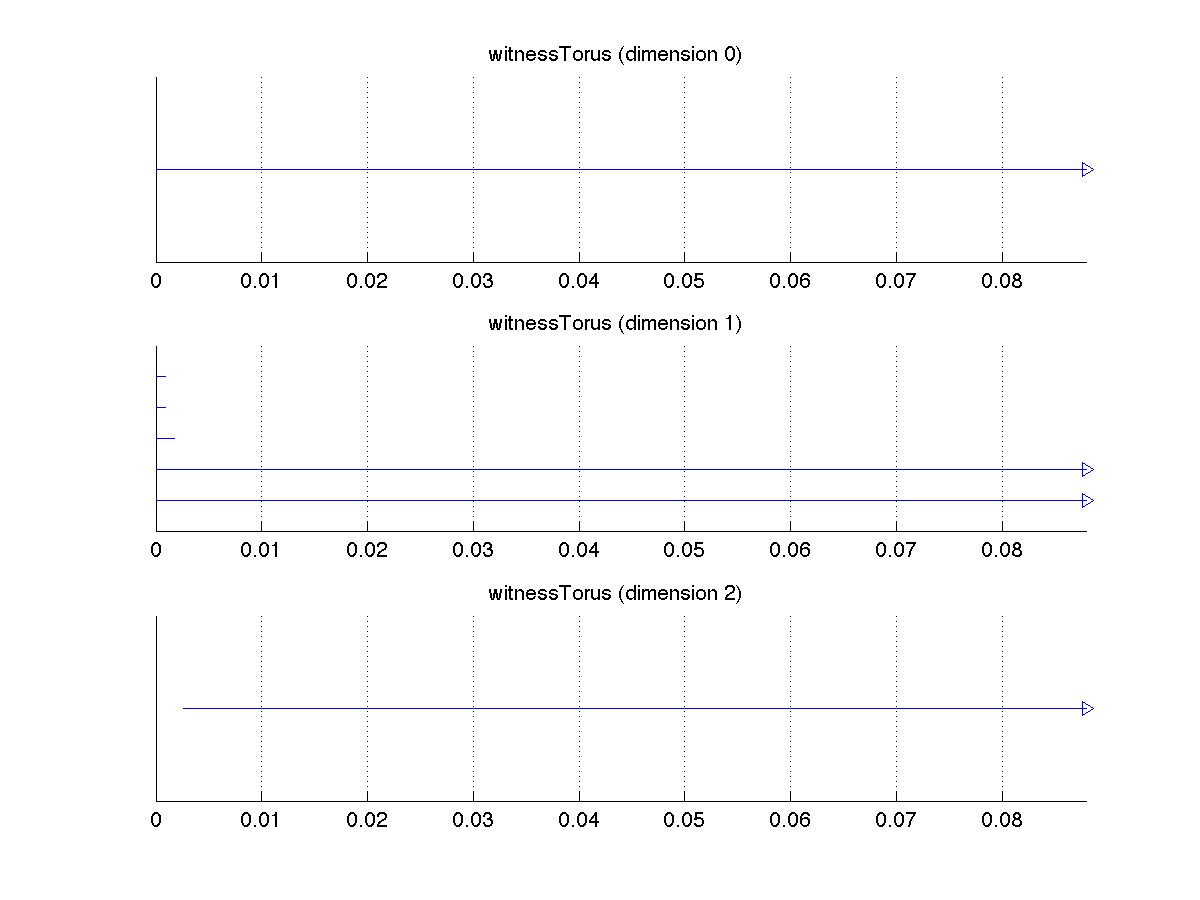
\includegraphics[width=6in]{witnessTorus.png}
   	\end{center}
\end{figure}
\FloatBarrier

The idea of persistent homology is that long intervals should correspond to real topological features, whereas short intervals are considered to be noise. The plot above shows that for a long range, the torus numbers $Betti_0 = 1$, $Betti_1 = 2$, $Betti_2 = 1$ are obtained. Your plot should contain a similar range.

The witness stream above contains approximately 2,000 simplices, fewer than the approximately 80,000 simplices in the Vietoris--Rips stream from the torus example in Section \ref{Vietoris--Rips}. This is despite the fact that we started with a point cloud of 100,000 points in the witness case, but of only 400 points in the Vietoris--Rips case. This supports our belief that the witness stream returns good results at lower computational expense. 


\subsection{Lazy witness streams}
A lazy witness stream is similar to a witness stream. However, there is an extra parameter $\nu$, typically chosen to be 0, 1, or 2, which helps determine how the lazy witness complexes $\LW_\nu(Z,L,t)$ are constructed. See \citet{WitnessComplexes} for more information. 

Suppose we are given a point cloud $Z$, landmark subset $L$, and parameter $\nu\in\mathbb{N}$. If $\nu = 0$, let $m(z) = 0$ for all $z\in Z$. If $\nu >0$, let $m(z)$ be the distance from $z$ to the $\nu$-th closest landmark point. The lazy witness complex $\LW_\nu(Z,L,t)$ is defined as follows.
\begin{itemize}
\item{the vertex set is $L$.}
\item{for vertices $a$ and $b$, edge $[ab]$ is in $\LW_\nu(Z,L,t)$ if there exists a witness $z \in Z$ such that $$\max\bigl\{d(a,z), d(b,z)\bigr\} \leq t+m(z).$$}
\item{a higher dimensional simplex is in $\LW_\nu(Z,L,t)$ if all of its edges are.} 
\end{itemize}
Note that $\LW_\nu(Z,L,t) \subset \LW_\nu(Z,L,s)$ whenever $t\leq s$. The adjective {\em lazy} refers to the fact that the lazy witness complex is a flag complex: since the 1-skeleton determines all higher dimensional simplices, less computation is involved. 

\begin{exercise}
Let $Z$ be the point cloud in Figure \ref{fig:housePointCloud} from Section \ref{euc}, corresponding to the house point cloud. Let $L = \{(1,0),(0,3),(-1,0)\}$ be the landmark subset. Let $\nu = 1$. Find by hand the filtration time for the edge between vertices $(1,0)$ and $(0,3)$. Which point or points witness this edge? What is the filtration time for the lone 2-simplex $[(1,0),(0,3),(-1,0)]$? 
\end{exercise}

\begin{exercise}
Repeat the above exercise with $\nu = 0$ and with $\nu = 2$. 
\end{exercise}

\begin{exercise}
Check that the 1-skeleton of a witness complex $\W(Z,L,t)$ is the same as the 1-skeleton of a lazy witness complex $\LW_2(Z,L,t)$. As a consequence, $\LW_2(Z,L,t)$ is the flag complex of $\W(Z,L,t)$. 
\end{exercise}

{\em 2-sphere example.} The Matlab script corresponding to this example is \href{https://github.com/javaplex/javaplex/tree/master/src/matlab/for_distribution/tutorial_examples/lazy_witness_example.m}{\texttt{lazy\_witness\_example.m}}.

We use parameter $\nu = 1$.

\begin{quote} \begin{verbatim}
>> max_dimension = 3;
>> num_points = 1000;
>> num_landmark_points = 50;
>> nu = 1;
>> num_divisions = 100;

>> point_cloud = examples.PointCloudExamples.getRandomSpherePoints(num_points, ...
max_dimension - 1);
>> landmark_selector = api.Plex4.createMaxMinSelector(point_cloud, num_landmark_points); 
\end{verbatim} \end{quote}

Often $t_{max}$ is chosen in proportion to \texttt{R}. 

% Is LazyWitnessStream constructer being added to class api?
\begin{quote} \begin{verbatim} 
>> R = landmark_selector.getMaxDistanceFromPointsToLandmarks()
R = 0.3841                         % Generally close to 0.38
>> max_filtration_value = 2 * R;
>> stream = streams.impl.LazyWitnessStream(landmark_selector.getUnderlyingMetricSpace(), ...
landmark_selector, max_dimension, max_filtration_value, nu, num_divisions); 
>> stream.finalizeStream()
>> num_simplices = stream.getSize()
num_simplices = 56518                         % Generally close to 50000
>> persistence = api.Plex4.getModularSimplicialAlgorithm(max_dimension, 2);
>> intervals = persistence.computeIntervals(stream);

>> options.filename = 'lazySphere';
>> options.max_filtration_value = max_filtration_value;
>> options.max_dimension = max_dimension - 1;
>> plot_barcodes(intervals, options);
\end{verbatim} \end{quote}

The file \texttt{lazySphere.png} is saved to your current directory.

\begin{figure}[htp]
	\begin{center}
    	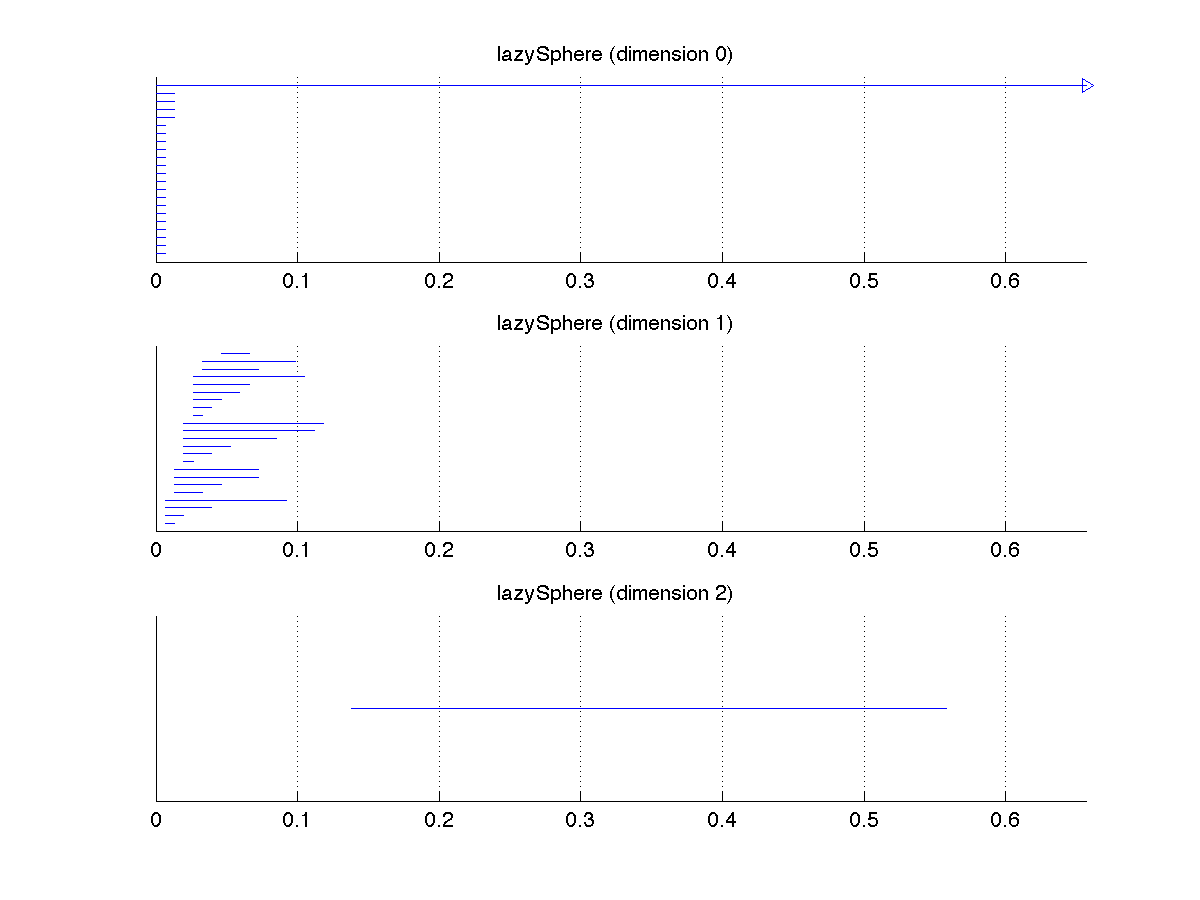
\includegraphics[width=6in]{lazySphere.png}
   	\end{center}
\end{figure}
\FloatBarrier

\begin{exercise}\label{Ex:flatTorusLazy}
In Exercise \ref{Ex:flatTorus} you created an explicit metric space for 1,000 random points on a flat torus. Build a lazy witness stream on this explicit metric space with 50 landmarks chosen via sequential maxmin and with $\nu = 1$.  Confirm the barcodes match the homology of a torus. 
\end{exercise}

\begin{exercise}\label{Ex:flatKleinLazy}
In Exercise \ref{Ex:flatTorus} you created an explicit metric space for 1,000 random points on a flat Klein bottle. Build a lazy witness stream on this explicit metric space with 50 landmarks chosen via sequential maxmin and with $\nu = 1$.  Confirm the barcodes match the homology of a Klein bottle, over $\mathbb{Z}_2$ and $\mathbb{Z}_3$ coefficients. 
\end{exercise}

\begin{exercise}\label{Ex:quotProjPlaneLazy}
In Exercise \ref{Ex:quotProjPlane} you created an explicit metric space for 1,000 random points on a projective plane. Build a lazy witness stream on this explicit metric space with 50 landmarks chosen via sequential maxmin and with $\nu = 1$.  Confirm the barcodes match the homology of a projective plane, over $\mathbb{Z}_2$ and $\mathbb{Z}_3$ coefficients. 
\end{exercise}
% This exercise was first done by David Eisenbud and Agnes Beadry at MRC.

\begin{exercise}
Sample points from an embedding of a double torus, that is, a surface of genus two, in $\mathbb{R}^3$. Build a lazy witness stream on this Euclidean metric space. Confirm the barcodes match the homology of a double torus. Choosing suitable parameters will not be easy.
\end{exercise}


\section{Example with real data}\label{real}

We now do an example with real data. The corresponding Matlab script is \href{https://github.com/javaplex/javaplex/tree/master/src/matlab/for_distribution/tutorial_examples/image_patch_example.m}{\texttt{image\_patch\_example.m}}, and it relies on the files \href{https://github.com/javaplex/javaplex/tree/master/src/matlab/for_distribution/tutorial_examples/pointsRange.mat}{\texttt{pointsRange.mat}} and \href{https://github.com/javaplex/javaplex/tree/master/src/matlab/for_distribution/tutorial_examples/dct.m}{\texttt{dct.m}}. 

In {\em On the nonlinear statistics of range image patches} \citep{Range}, we study a space of range image patches drawn from the Brown database \citep{Mumford}. A range image is like an optical image, except that each pixel contains a distance instead of a grayscale value. Our space contains high-contrast, normalized, $5 \times5$ pixel patches. We write each $5\times5$ patch as a vector with 25 coordinates and think of our patches as point cloud data in $\mathbb{R}^{25}$. We select from this space the 30\% densest vectors, based on a density estimator called $\rho_{300}$ (see Appendix \ref{A:core}). In \citet{Range} this dense core subset is denoted $X^5(300,30)$, and it contains 15,000 points. In the next example we verify a result from \citet{Range}: $X^5(300,30)$ has the topology of a circle. 

Load the file \href{https://github.com/javaplex/javaplex/tree/master/src/matlab/for_distribution/tutorial_examples/pointsRange.mat}{\texttt{pointsRange.mat}}. The matrix \texttt{pointsRange} appears in your Matlab workspace.

\begin{quote} \begin{verbatim}
>> load pointsRange.mat
>> size(pointsRange) 
ans = 15000    25                         % 15000 points in dimension 25
\end{verbatim} \end{quote}

Matrix \texttt{pointsRange} is in fact $X^5(300,30)$: each of its rows is a vector in $\mathbb{R}^{25}$. Display some of the coordinates of \texttt{pointsRange}. It is not easy to visualize a circle by looking at these coordinates! 

We pick 50 sequential maxmin landmark points, we find the value of \texttt{R}, and we build the lazy witness stream with parameter $\nu = 1$. 

\begin{quote} \begin{verbatim}
>> max_dimension = 3;
>> num_landmark_points = 50;
>> nu = 1;
>> num_divisions = 500;

>> landmark_selector = api.Plex4.createMaxMinSelector(pointsRange, num_landmark_points);
>> R = landmark_selector.getMaxDistanceFromPointsToLandmarks() 
R = 0.7759                         % Generally close to 0.75
>> max_filtration_value = R / 3;
>> stream = streams.impl.LazyWitnessStream(landmark_selector.getUnderlyingMetricSpace(), ...
landmark_selector, max_dimension, max_filtration_value, nu, num_divisions);
>> stream.finalizeStream()
>> num_simplices = stream.getSize()
num_simplices = 12036                         % Generally between 10000 and 25000

>> persistence = api.Plex4.getModularSimplicialAlgorithm(max_dimension, 2);
>> intervals = persistence.computeIntervals(stream);

>> options.filename = 'lazyRange';
>> options.max_filtration_value = max_filtration_value;
>> options.max_dimension = max_dimension - 1;
>> plot_barcodes(intervals, options);
\end{verbatim} \end{quote}

The file \texttt{lazyRange.png} is saved to your current directory.

\begin{figure}[htp]
	\begin{center}
    	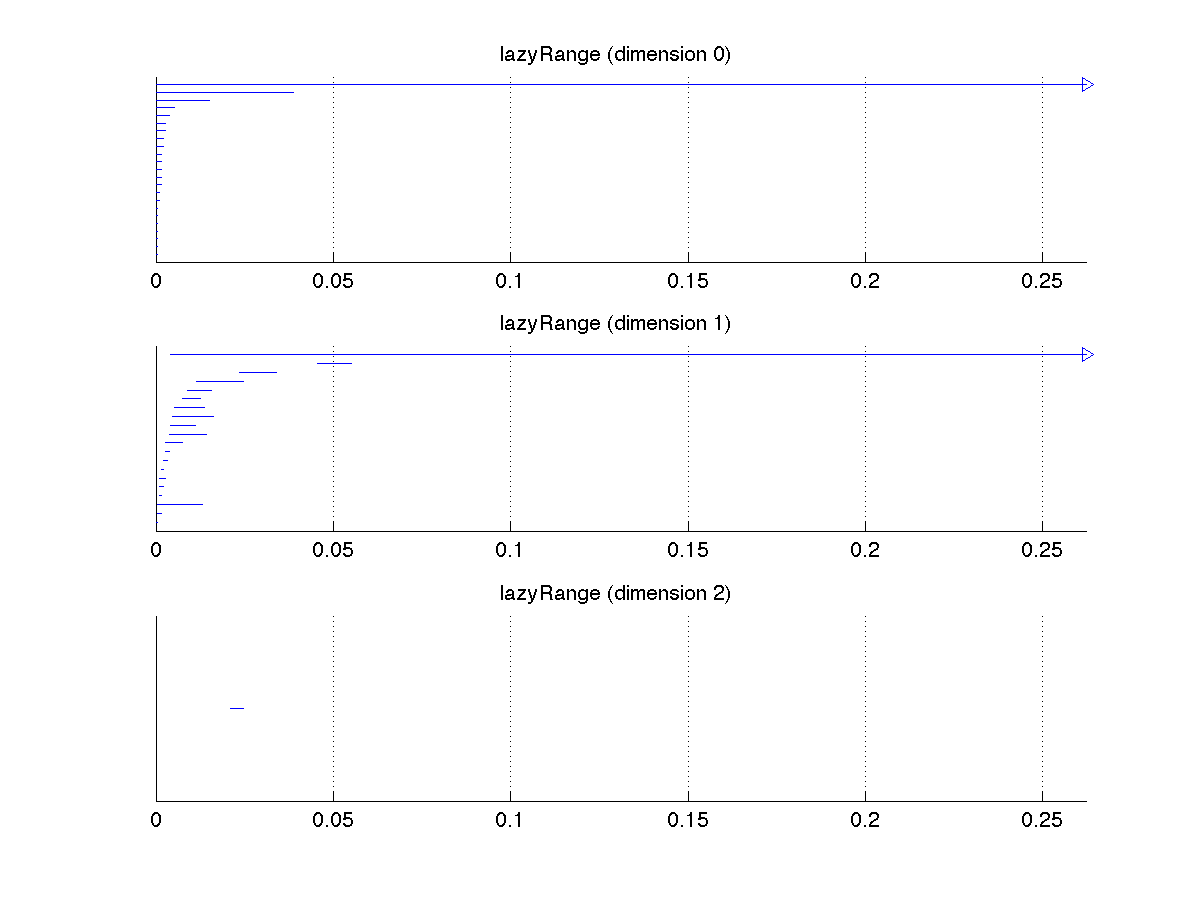
\includegraphics[width=6in]{lazyRange.png}
   	\end{center}
	\caption{Betti intervals for the lazy witness complex built from $X^5(300,30)$}
  	\label{fig:rangeBetti}
\end{figure}
\FloatBarrier

The plots above show that for a long range, the circle Betti numbers $Betti_0 = Betti_1 = 1$ are obtained. Your plot should contain a similar range. This is good evidence that the core subset $X^5(300,30)$ is well-approximated by a circle. 

Our $5\times 5$ normalized patches are currently in the pixel basis: every coordinate corresponds to the range value at one of the 25 pixels. The Discrete Cosine Transform (DCT) basis is a useful basis for our patches \citep{Range, Mumford}. We change to this basis in order to plot a projection of the loop evidenced by Figure \ref{fig:rangeBetti}. The method \href{https://github.com/javaplex/javaplex/tree/master/src/matlab/for_distribution/tutorial_examples/dct.m}{\texttt{dct.m}} returns the DCT change-of-basis matrix for square patches of size specified by the input parameter.

%>> size(pointsRangeDct)
%ans = 15000\quad 24 \hspace{30mm} \% 15000 points in DCT basis (representation)
\begin{quote} \begin{verbatim} 
>> pointsRangeDct = pointsRange * dct(5);
\end{verbatim} \end{quote}

Two of the DCT basis vectors are horizontal and linear gradients.

\vspace{-3mm}
\begin{figure}[htb]
	\centering
	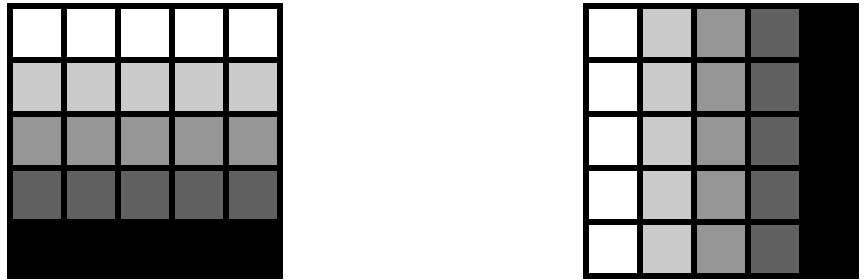
\includegraphics[width=2in]{linearGrad}
\end{figure}
\vspace{-3mm}
\FloatBarrier

We plot the projection of \texttt{pointsRangeDct} onto the linear gradient DCT basis vectors.

\begin{quote} \begin{verbatim}
>> scatter(pointsRangeDct(:,1), pointsRangeDct(:,5), '.')
>> axis square
\end{verbatim} \end{quote}

\begin{figure}[htp]
  \begin{center}
    \subfigure[Projection of $X^5(300,30)$]{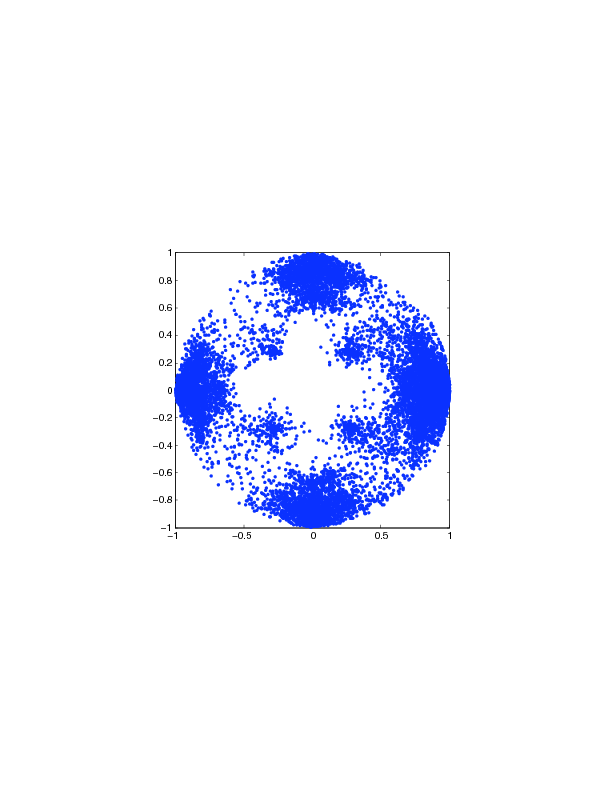
\includegraphics[width=3.0in]{r5k300c30}}
    \quad
    \subfigure[Range primary circle]{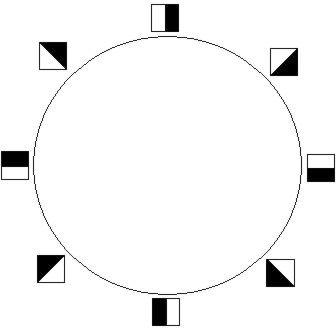
\includegraphics[width=2.9in]{primaryCircle}}
   \end{center}
\end{figure}
\FloatBarrier

The projection of $X^5(300,30)$ in Figure (a) shows a circle. It is called the range primary circle and is parameterized as shown in Figure (b).




\section{Remarks} 


\subsection{Matlab functions with javaPlex commands}\label{matlabFunctions}
Writing Matlab functions is very useful. In order to include javaPlex commands in an m-file function, include the command \texttt{import edu.stanford.math.plex4.*;} as the second line of the function ---  that is, as the first line underneath the function header. We include the m-file \href{https://github.com/javaplex/javaplex/tree/master/src/matlab/for_distribution/tutorial_examples/eulerCharacteristic.m}{\texttt{eulerCharacteristic.m}} as an example Matlab function.

{\em Euler characteristic example.}
The corresponding Matlab script is \href{https://github.com/javaplex/javaplex/tree/master/src/matlab/for_distribution/tutorial_examples/euler_characteristic_example.m}{\texttt{euler\_characteristic\_example.m}}, and it relies on the file \href{https://github.com/javaplex/javaplex/tree/master/src/matlab/for_distribution/tutorial_examples/eulerCharacteristic.m}{\texttt{eulerCharacteristic.m}}. 

First we create a 6-dimensional sphere. 

\begin{quote} \begin{verbatim}
>> dimension = 6;
>> stream = api.Plex4.createExplicitSimplexStream();
>> stream.addElement(0:(dimension + 1));
>> stream.ensureAllFaces();
>> stream.removeElementIfPresent(0:(dimension + 1));
>> stream.finalizeStream();
\end{verbatim} \end{quote}

The function \href{https://github.com/javaplex/javaplex/tree/master/src/matlab/for_distribution/tutorial_examples/eulerCharacteristic.m}{\texttt{eulerCharacteristic.m}} accepts an explicit simplex stream and its dimension as input. The function demonstrates two different methods for computing the Euler characteristic.

\begin{quote} \begin{verbatim}
>> eulerCharacteristic(stream, dimension)
The Euler characteristic is 2 = 8 - 28 + 56 - 70 + 56 - 28 + 8, using the alternating 
sum of cells.
The Euler characteristic is 2 = 1 - 0 + 0 - 0 + 0 - 0 + 1, using the alternating sum 
of Betti numbers.
\end{verbatim} \end{quote}


\subsection{Displaying the simplices in a stream}

It is possible to display the simplices in a stream, along with their filtration times. You can also obtain the vertices of each simplex as a Matlab matrix. For an example of how to do this, please see the file \href{https://github.com/javaplex/javaplex/blob/master/src/matlab/for_distribution/basic_examples/dump_example.m}{\texttt{dump\_example.m}} in the folder \href{https://github.com/javaplex/javaplex/tree/master/src/matlab/for_distribution/basic_examples}{\texttt{basic\_examples}}.


\subsection{Computing the bottleneck distance}

It is possible to compute the bottleneck distance between two barcodes. For an example of how to do this, please see the file \href{https://github.com/javaplex/javaplex/tree/master/src/matlab/for_distribution/tutorial_examples/bottleneck_distance_example.m}{\texttt{bottleneck\_distance\_example.m}} in the folder \href{https://github.com/javaplex/javaplex/tree/master/src/matlab/for_distribution/tutorial_examples}{\texttt{tutorial\_examples}}.


%\subsection{Java heap size}
%Depending on the size of your javaPlex computations, you may need to increase the maximum Java heap size. This should not be necessary for the examples in this tutorial. 

%The following command returns your maximum heap size in bytes.
%\begin{quote} \begin{verbatim} 
%>> java.lang.Runtime.getRuntime.maxMemory
%ans = 130875392
%\end{verbatim} \end{quote}
%My computer has a heap limit of approximately 128 megabytes. To increase your limit to, say, 256 megabytes, create a file named \texttt{java.opts} in your Matlab directory which contains the text \texttt{-Xmx256m} and then restart Matlab.


%\subsection{From Java variables to Matlab variables}
%Some javaPlex commands return Java variables, when instead one might want output in the form of a Matlab variable, such as a matrix of numbers. One way to transform Java variables into Matlab variables is by using an m-file. For instance, in Section ?? %\ref{explicitStream} 
% no
%we used the m-file \texttt{interval2mat.m} to take an array of type PersistenceInterval into a Matlab matrix. Similarly, the m-file \texttt{betti2mat.m} accepts input of type \texttt{Plex.BettiNumbers} and returns a Matlab vector of integers. These commands are typically used as shown below, where \texttt{intervals} is an array of type PersistenceInterval.

%\begin{quote} \begin{verbatim} intervalMatrix = interval2mat(intervals);
%>> bettiVect = betti2vect(Plex.FilterInfinite(intervals)); 
%\end{verbatim} \end{quote}




\appendix
\appendixpage
\addappheadtotoc




\section{Dense core subsets}\label{A:core}

A core subset of a dataset is a collection of the densest points, such as $X^5(300,30)$ in Section \ref{real}. Since there are many density estimators, and since we can choose any number of the densest points, a dataset has a variety of core subsets. In this appendix we discuss how to create core subsets. 

Real datasets can be very noisy, and outlier points can significantly alter the computed topology. Therefore, instead of trying to approximate the topology of an entire dataset, we often proceed as follows. We create a family of core subsets and identify their topologies. Looking at a variety of core subsets can give a good picture of the entire dataset. 

See \citet{KleinBottle} and \citet{WitnessComplexes} for an example using multiple core subsets. The dataset contains high-contrast patches from natural images. The authors use three density estimators. As they change from the most global to the most local density estimate, the topologies of the core subsets change from a circle, to three intersecting circles, to a Klein bottle. 

One way to estimate the density of a point $z$ in a point cloud $Z$ is as follows. Let $\rho_k(z)$ be the distance from $z$ to its $k$-th closest neighbor. Let the density estimate at $z$ be $\frac{1}{\rho_k(z)}$. Varying parameter $k$ gives a family of density estimates. Using a small value for $k$ gives a local density estimate, and using a larger value for $k$ gives a more global estimate. 

For Euclidean datasets, one can use the m-file \href{https://github.com/javaplex/javaplex/tree/master/src/matlab/for_distribution/tutorial_examples/kDensitySlow.m}{\texttt{kDensitySlow.m}} to produce density estimates $\frac{1}{\rho_k}$. The following command is typical.

\begin{quote} \begin{verbatim}
>> densities = kDensitySlow(points, k); 
\end{verbatim} \end{quote}

Input \texttt{points} is an $N\times n$ matrix of $N$ points in $\mathbb{R}^n$. Input $k$ is the density estimate parameter. Output \texttt{densities} is a vertical vertex of length $N$ containing the density estimate at each point. 

M-file \href{https://github.com/javaplex/javaplex/tree/master/src/matlab/for_distribution/tutorial_examples/coreSubset.m}{\texttt{coreSubset.m}} builds a core subset. The following command is typical.

\begin{quote} \begin{verbatim}
>> core = coreSubset(points, densities, numPoints); 
\end{verbatim} \end{quote}

Inputs \texttt{points} and \texttt{densities} are as above. Output \texttt{core} is a $\texttt{numPoints}\times n$ matrix representing the \texttt{numPoints} densest points. 

{\em Prime numbers example.} The Matlab script corresponding to this example is \href{https://github.com/javaplex/javaplex/tree/master/src/matlab/for_distribution/tutorial_examples/core_subsets_example.m}{\texttt{core\_subsets\_example.m}}.

The command \texttt{primes(3571)} returns a vector listing all prime numbers less than or equal to 3571, which is the 500-th prime. We think of these primes as points in $\mathbb{R}$ and build the core subset of the 10 densest points with density parameter $k = 1$.
\begin{quote} \begin{verbatim} 
>> p = primes(3571)';
>> length(p)
ans = 500
>> densities1 = kDensitySlow(p, 1);
>> core1 = coreSubset(p, densities1, 10)
core1 =

    2
    3
    5
    7
    11
    13
    17
    19
    29
    31
\end{verbatim} \end{quote}

We get a bunch of twin primes, which makes sense since $k = 1$. Let's repeat with $k = 50$.

\begin{quote} \begin{verbatim}
>> densities50 = kDensitySlow(p, 50);
>> core50 = coreSubset(p, densities50, 10)
core50 =

    113
    127
    109
    131
    107
    137
    139
    157
    149
    151
\end{verbatim} \end{quote}
 
With $k = 50$, we expect the densest points to be slightly larger than the 25-th prime, which is 97. 

{\em Note:} As its name suggests, the m-file \href{https://github.com/javaplex/javaplex/tree/master/src/matlab/for_distribution/tutorial_examples/kDensitySlow.m}{\texttt{kDensitySlow.m}} is not the most efficient way to calculate $\rho_k$ for large datasets. There is a faster file \texttt{kDensity.m} for this purpose, which uses the kd-tree data structure. It is not included in the tutorial because it requires one to download a kd-tree package for Matlab, available at \url{http://www.mathworks.com/matlabcentral/fileexchange/21512-kd-tree-for-matlab}. Please email Henry at \texttt{henrya@ima.umn.edu} if you're interested in using \texttt{kDensity.m}. 

% What are the differences in timings between fast and slow versions?
% It seems that k=300 is surprisingly slow with kDensity.m: 1108 seconds. Slower than kDensitySlow.m. Double check?

%I typically use the m-file \texttt{kDensitySlow.m} on datasets of around 50,000 points (for instance, $X^5(300,30)$ in Section \ref{real} is the 30\% densest points from a set of size 50,000, using the density estimate $\rho_{300}$). This computation takes about 10 minutes on my MacBook, which is much longer than any of the computations I do using the JPlex software.  % Elapsed time is 432.024880 seconds, 7-17-09. This was effectively kDensitySlow.m, I think




\section{Exercise solutions}\label{A:solutions}

Several exercise solutions are accompanied by Matlab scripts, which are available in the folder \href{https://github.com/javaplex/javaplex/tree/master/src/matlab/for_distribution/tutorial_solutions}{\texttt{tutorial\_solutions}}.

\begin{exerciseSol}
Build a simplicial complex homeomorphic to the torus. Compute its Betti numbers. {\em Hint: You will need at least 7 vertices} \citep[page 107]{Hatcher}{\em . We recommend using a $3\times 3$ grid of 9 vertices.}
\end{exerciseSol}

\begin{solution}
See the Matlab script \href{https://github.com/javaplex/javaplex/tree/master/src/matlab/for_distribution/tutorial_solutions/exercise_1.m}{\texttt{exercise\_1.m}} in folder \href{https://github.com/javaplex/javaplex/tree/master/src/matlab/for_distribution/tutorial_solutions}{\texttt{tutorial\_solutions}} for a solution. We use 9 vertices, which we think of as a $3 \times 3$ grid numbered as a telephone keypad. We identify opposite sides.
\end{solution}

\begin{figure}[htp]
  \begin{center}
    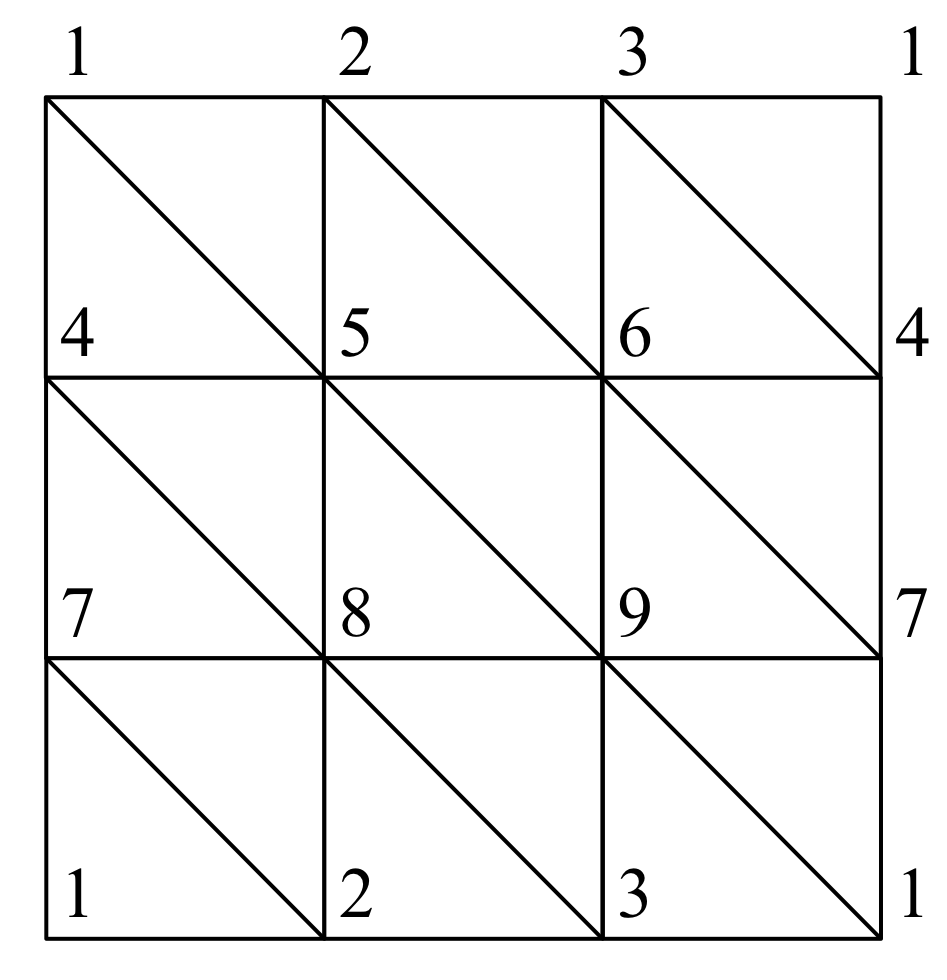
\includegraphics[width=2.5in]{torus}
   \end{center}
\end{figure}
\FloatBarrier

\begin{exerciseSol}
Build a simplicial complex homeomorphic to the Klein bottle. Check that it has the same Betti numbers as the torus over $\mathbb{Z}_2$ coefficients but different Betti numbers over $\mathbb{Z}_3$ coefficients.
\end{exerciseSol}

\begin{solution}
See the Matlab script \href{https://github.com/javaplex/javaplex/tree/master/src/matlab/for_distribution/tutorial_solutions/exercise_2.m}{\texttt{exercise\_2.m}} for a solution. We use 9 vertices, which we think of as a $3 \times 3$ grid numbered as a telephone keypad. We identify opposite sides, with left and right sides identified with a twist. 
\end{solution}

\begin{figure}[htp]
  \begin{center}
    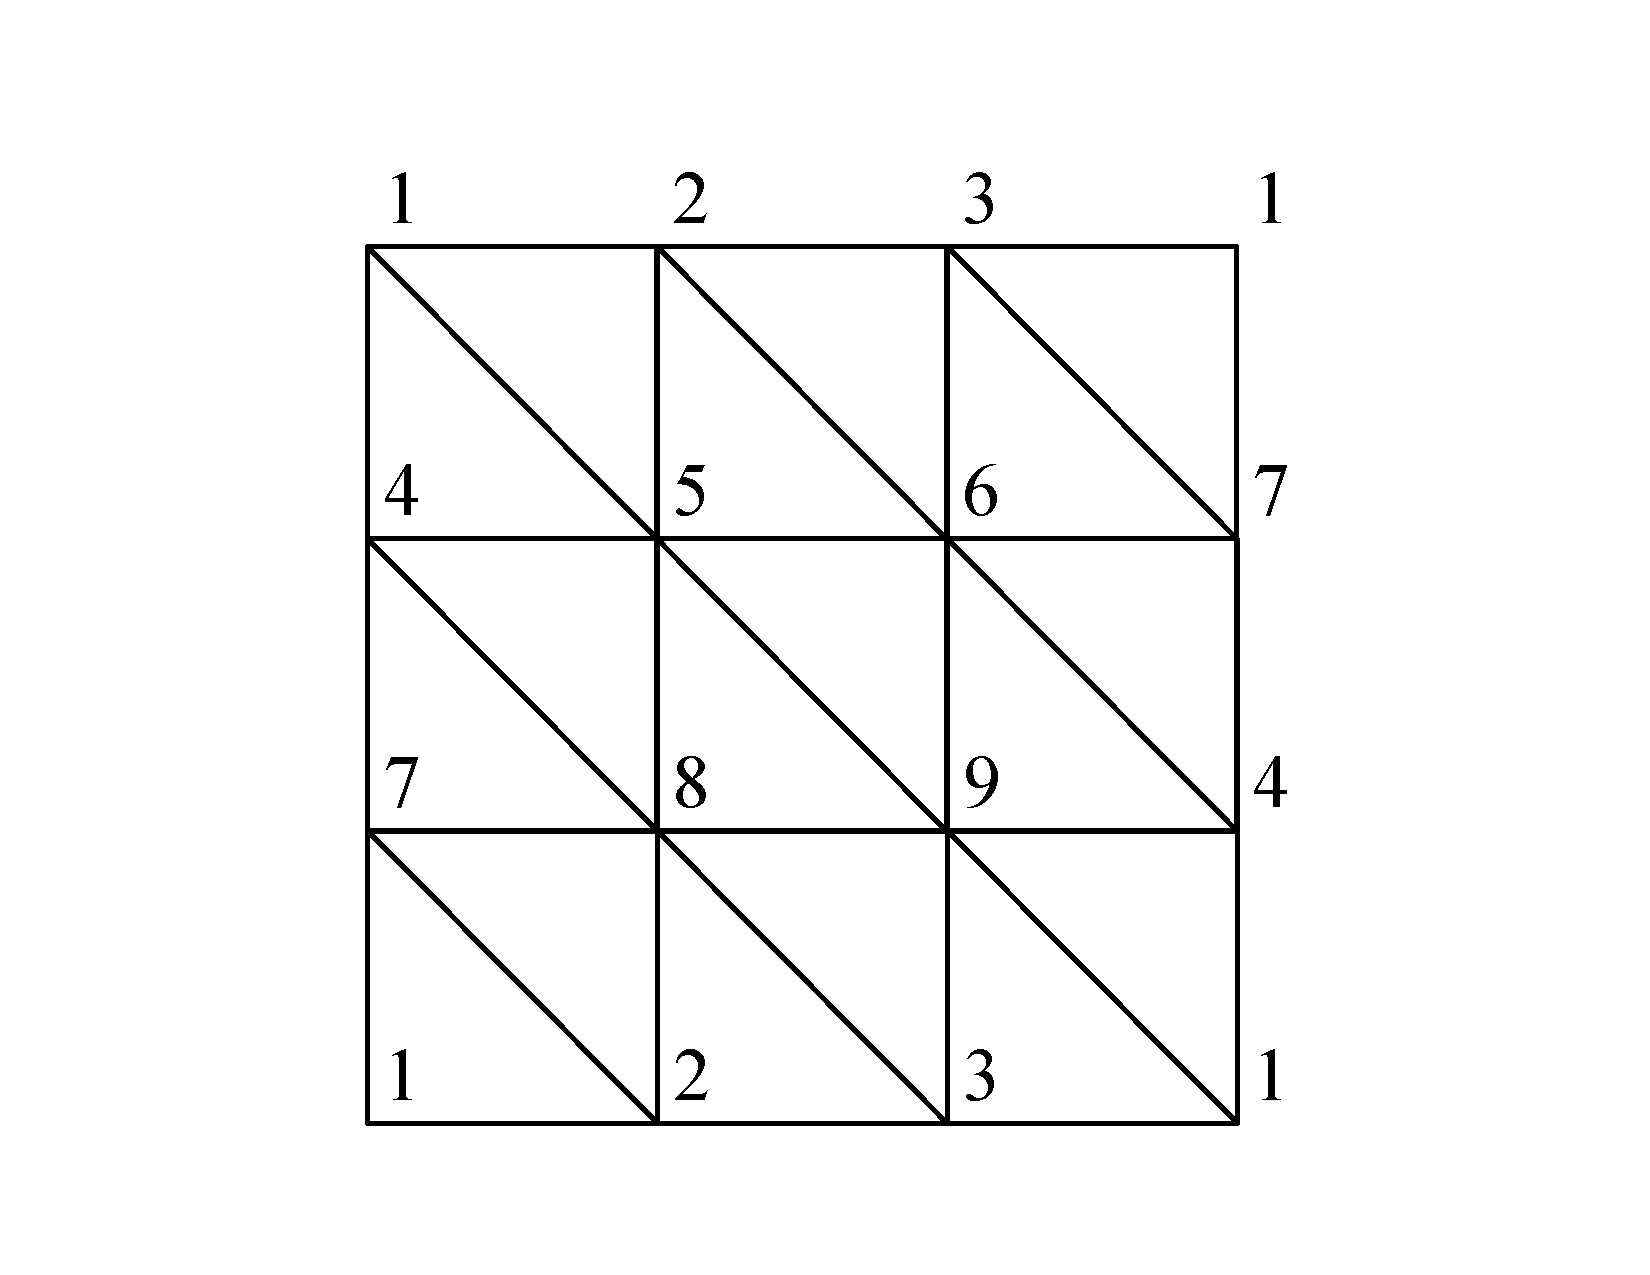
\includegraphics[width=2.5in]{klein}
   \end{center}
\end{figure}
\FloatBarrier

\begin{exerciseSol}
Build a simplicial complex homeomorphic to the projective plane. Find its Betti numbers over $\mathbb{Z}_2$ and $\mathbb{Z}_3$ coefficients.
\end{exerciseSol}

\begin{solution}
See the Matlab script \href{https://github.com/javaplex/javaplex/tree/master/src/matlab/for_distribution/tutorial_solutions/exercise_3.m}{\texttt{exercise\_3.m}} for a solution. We use the minimal triangulation for the projective plane, which contains 6 vertices.
\end{solution}

\begin{figure}[htp]
  \begin{center}
    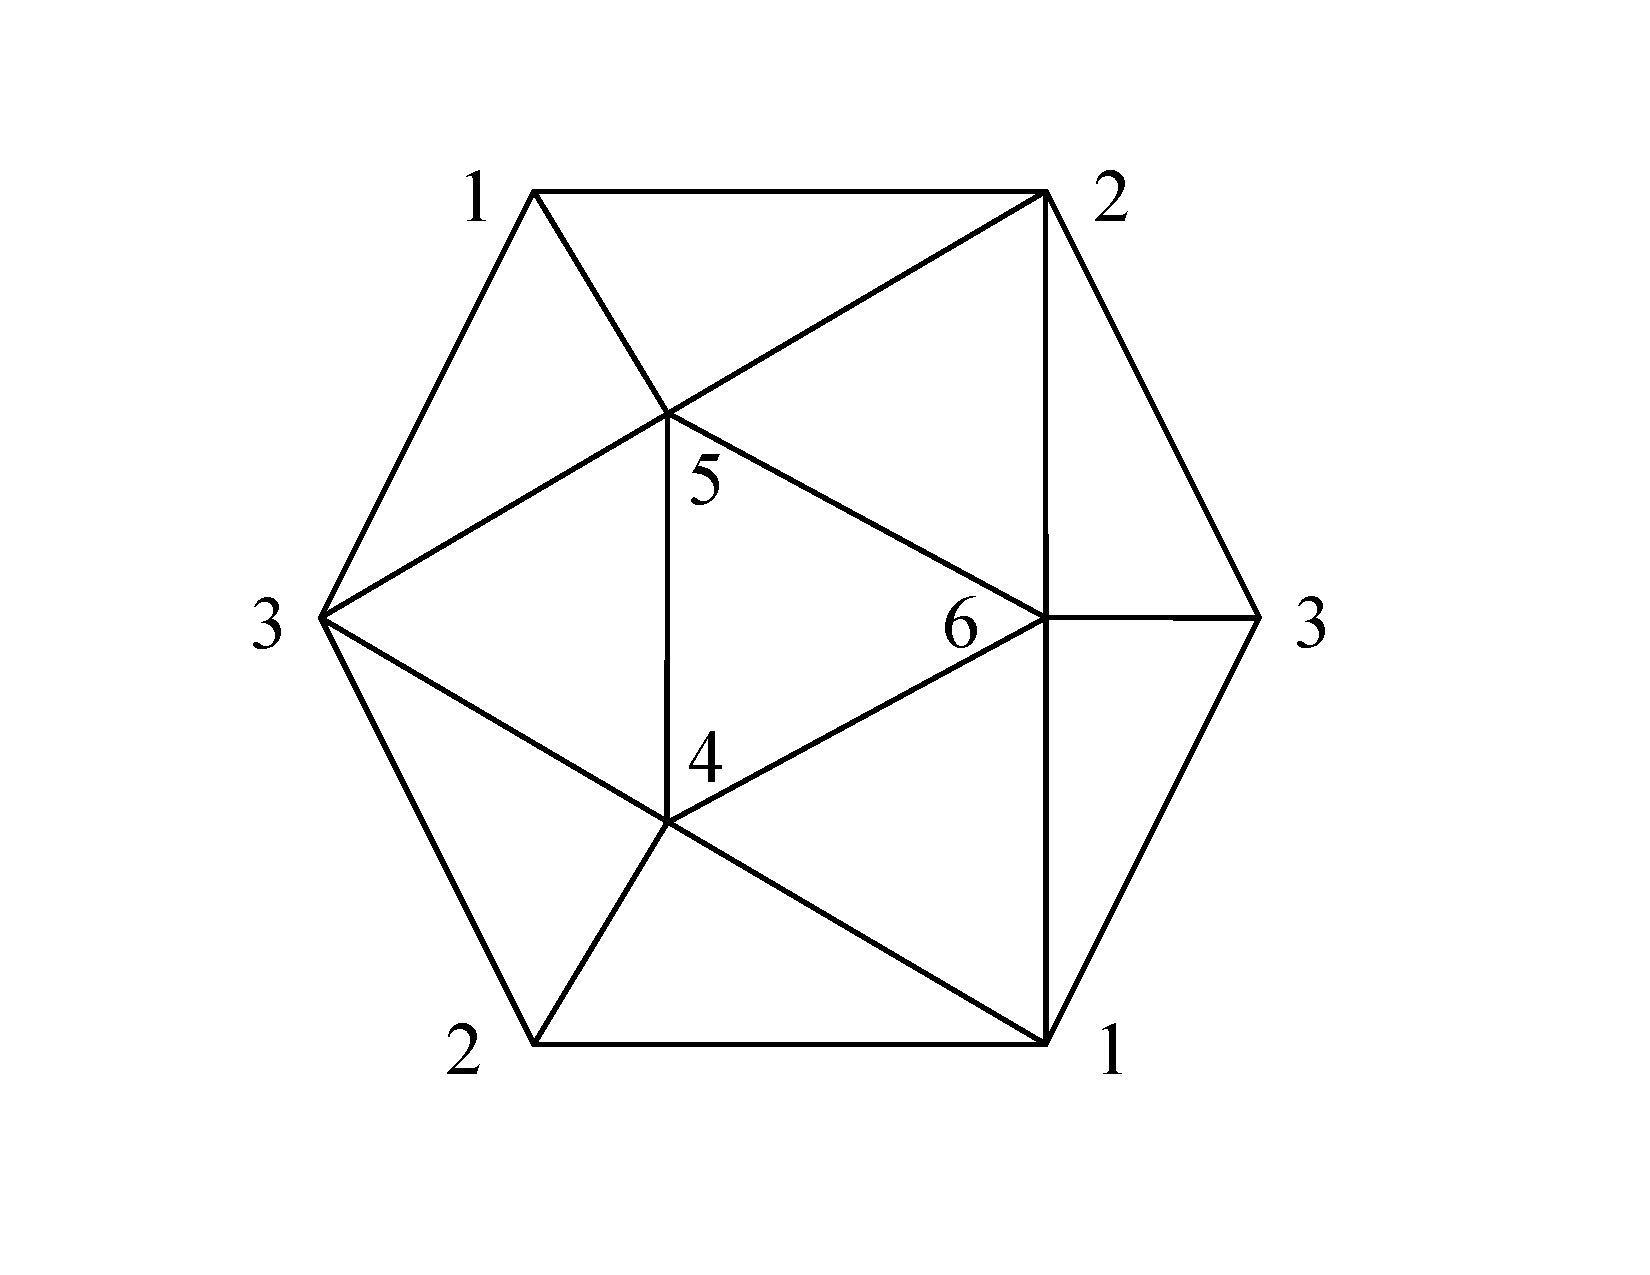
\includegraphics[width=2.5in]{projPlane}
   \end{center}
\end{figure}
\FloatBarrier

\begin{exerciseSol}
Write a Matlab script or function that selects 1,000 random points from the square $[0, 1] \times [0, 1]$ and then computes the 1,000 $\times$ 1,000 distance matrix for these points under the induced metric on the flat torus. Create an explicit metric space from this distance matrix.
\end{exerciseSol}

\begin{solution}
See the Matlab script \href{https://github.com/javaplex/javaplex/tree/master/src/matlab/for_distribution/tutorial_solutions/exercise_4.m}{\texttt{exercise\_4.m}} and the Matlab function \href{https://github.com/javaplex/javaplex/tree/master/src/matlab/for_distribution/tutorial_solutions/flatTorusDistanceMatrix.m}{\texttt{flatTorusDistanceMatrix.m}} for a solution.
\end{solution}

\begin{exerciseSol}
Write a Matlab script or function that selects 1,000 random points from the square $[0, 1] \times [0, 1]$ and then computes the 1,000 $\times$ 1,000 distance matrix for these points under the induced metric on the flat Klein bottle. Create an explicit metric space from this distance matrix.
\end{exerciseSol}

\begin{solution}
See the Matlab script \href{https://github.com/javaplex/javaplex/tree/master/src/matlab/for_distribution/tutorial_solutions/exercise_5.m}{\texttt{exercise\_5.m}} and the Matlab function \href{https://github.com/javaplex/javaplex/tree/master/src/matlab/for_distribution/tutorial_solutions/flatKleinDistanceMatrix.m}{\texttt{flatKleinDistanceMatrix.m}} for a solution.
\end{solution}

\begin{exerciseSol}
Write a Matlab script or function that selects 1,000 random points from the unit sphere $S^2 \subset \mathbb{R}^3$ and then computes the 1,000 $\times$ 1,000 distance matrix for these points under the induced metric on the projective plane. Create an explicit metric space from this distance matrix. 
\end{exerciseSol}

\begin{solution}
See the Matlab script \href{https://github.com/javaplex/javaplex/tree/master/src/matlab/for_distribution/tutorial_solutions/exercise_6.m}{\texttt{exercise\_6.m}} and the Matlab function \href{https://github.com/javaplex/javaplex/tree/master/src/matlab/for_distribution/tutorial_solutions/projPlaneDistanceMatrix.m}{\texttt{projPlaneDistanceMatrix.m}} for a solution.
\end{solution}

\begin{exerciseSol}
Slowly increase the values for $t_{max}$, $d_{max}$ and note how quickly the size of the Vietoris--Rips stream and the time of computation grow. Either increasing $t_{max}$ from 0.9 to 1 or increasing $d_{max}$ from 3 to 4 roughly doubles the size of the Vietoris--Rips stream.
\end{exerciseSol}

\begin{solution}
No solution included. 
\end{solution}

\begin{exerciseSol}
Find a planar dataset $Z \subset \mathbb{R}^2$ and a filtration value $t$ such that $\VR(Z,t)$ has nonzero $Betti_2$. Build a Vietoris--Rips stream to confirm your answer.
\end{exerciseSol}

\begin{solution}
See the Matlab script \href{https://github.com/javaplex/javaplex/tree/master/src/matlab/for_distribution/tutorial_solutions/exercise_8.m}{\texttt{exercise\_8.m}} for a solution. Our planar dataset is 6 evenly spaced points on the unit circle. We build a Vietoris--Rips stream which, at the correct filtration value, is an octahedron. 
\end{solution}

\begin{exerciseSol}
Find a planar dataset $Z \subset \mathbb{R}^2$ and a filtration value $t$ such that $\VR(Z,t)$ has nonzero $Betti_6$. When building a Vietoris--Rips stream to confirm your answer, don't forget to choose $d_{max} = 7$.
\end{exerciseSol}

\begin{solution}
See the Matlab script \href{https://github.com/javaplex/javaplex/tree/master/src/matlab/for_distribution/tutorial_solutions/exercise_9.m}{\texttt{exercise\_9.m}} for a solution. Our planar dataset is 14 evenly spaced points on the unit circle. We build a Vietoris--Rips stream which, at the correct filtration value, is homeomorphic to the 6-sphere. It has 14 vertices because it is obtained by suspending the 0-sphere six times, for a total of $2 + (6 \times 2) = 14$ vertices. 
\end{solution}

\begin{exerciseSol}
Let $Z$ be the point cloud in Figure \ref{fig:housePointCloud} from Section \ref{euc}, corresponding to the house point cloud. Suppose we are using sequential maxmin to select a set $L$ of 3 landmarks, and the first (randomly selected) landmark is $(1,0)$. Find by hand the other two landmarks in $L$.
\end{exerciseSol}

\begin{solution}
$L$ is the set $\{(1, 0), (0, 3), (-1, 0)\}$. 
\end{solution}

\begin{exerciseSol}
Let $Z$ be a point cloud and $L$ a landmark subset. Show that if $L$ is chosen via sequential maxmin, then for any $l_i,l_j\in L$, we have $d(l_i,l_j)\geq\texttt{R}$.
\end{exerciseSol}

\begin{solution}
Without loss of generality, assume that $i < j$ and that landmarks $l_i$ and $l_j$ were the $i$-th and $j$-th landmarks selected by the inductive sequential maxmin process. Let $L_{j-1}$ be the first $j - 1$ landmarks chosen. 

We proceed using a proof by contradiction. Suppose that $d(l_i, l_j) < \texttt{R}$. By definition of \texttt{R}, there exists a $z \in Z$ such that $d(z,L) = \texttt{R}$. Note that
$$d(l_j, L_{j-1}) \leq d(l_j, l_i) = d(l_i, l_j) < \texttt{R} = d(z,L) \leq d(z, L_{j-1}).$$
This contradicts the fact that landmark $l_j$ was chosen at the $j$-th step of sequential maxmin. Hence, it must be the case that $d(l_i, l_j) \geq \texttt{R}$. 
\end{solution}

\begin{exerciseSol}
Let $Z$ be the point cloud in Figure \ref{fig:housePointCloud} from Section \ref{euc}, corresponding to the house point cloud. Let $L = \{(1,0),(0,3),(-1,0)\}$ be the landmark subset. Find by hand the filtration time for the edge between vertices $(1,0)$ and $(0,3)$. Which point or points witness this edge? What is the filtration time for the lone 2-simplex $[(1,0),(0,3),(-1,0)]$?
\end{exerciseSol}

\begin{solution}
The edge between $(1, 0)$ and $(0, 3)$ has filtration time zero. Points $(1, 2)$ or $(0, 3)$ witness this edge. The lone 2-simplex has filtration time zero. 
\end{solution}

\begin{exerciseSol}
Let $Z$ be the point cloud in Figure \ref{fig:housePointCloud} from Section \ref{euc}, corresponding to the house point cloud. Let $L = \{(1,0),(0,3),(-1,0)\}$ be the landmark subset. Let $\nu = 1$. Find by hand the filtration time for the edge between vertices $(1,0)$ and $(0,3)$. Which point or points witness this edge? What is the filtration time for the lone 2-simplex $[(1,0),(0,3),(-1,0)]$?
\end{exerciseSol}

\begin{solution}
The edge between $(1, 0)$ and $(0, 3)$ has filtration time $2-\sqrt{2}$. Point $(1, 2)$ witnesses this edge. The lone 2-simplex has filtration time $\sqrt{2}$, which is when the edge between $(1, 0)$ and $(-1, 0)$ appears. 
\end{solution}

\begin{exerciseSol}
Repeat the above exercise with $\nu = 0$ and with $\nu = 2$.
\end{exerciseSol}

\begin{solution}
First we do the case when $\nu = 0$. The edge between $(1, 0)$ and $(0, 3)$ has filtration time 2. Point $(1, 2)$ witnesses this edge. The lone 2-simplex has filtration time 2. 

Next we do the case when $\nu = 2$. The edge between $(1, 0)$ and $(0, 3)$ has filtration time zero. Points $(1, 2)$ or $(0, 3)$ witness this edge. The lone 2-simplex has filtration time zero. 
\end{solution}

\begin{exerciseSol}
Check that the 1-skeleton of a witness complex $\W(Z,L,t)$ is the same as the 1-skeleton of a lazy witness complex $\LW_2(Z,L,t)$. As a consequence, $\LW_2(Z,L,t)$ is the flag complex of $\W(Z,L,t)$.
\end{exerciseSol}

\begin{solution}
This follows from the definition of the witness stream and the definition of the lazy witness stream for $\nu = 2$. 
\end{solution}

\begin{exerciseSol}
In Exercise \ref{Ex:flatTorus} you created an explicit metric space for 1,000 random points on a flat torus. Build a lazy witness stream on this explicit metric space with 50 landmarks chosen via sequential maxmin and with $\nu = 1$.  Confirm the barcodes match the homology of a torus. 
\end{exerciseSol}

\begin{solution}
See the Matlab script \href{https://github.com/javaplex/javaplex/tree/master/src/matlab/for_distribution/tutorial_solutions/exercise_16.m}{\texttt{exercise\_16.m}} and the Matlab function \href{https://github.com/javaplex/javaplex/tree/master/src/matlab/for_distribution/tutorial_solutions/flatTorusDistanceMatrix.m}{\texttt{flatTorusDistanceMatrix.m}} for a solution.
\end{solution}

\begin{exerciseSol}
In Exercise \ref{Ex:flatKlein} you created an explicit metric space for 1,000 random points on a flat Klein bottle. Build a lazy witness stream on this explicit metric space with 50 landmarks chosen via sequential maxmin and with $\nu = 1$.  Confirm the barcodes match the homology of a Klein bottle, over $\mathbb{Z}_2$ and $\mathbb{Z}_3$ coefficients.
\end{exerciseSol}

\begin{solution}
See the Matlab script \href{https://github.com/javaplex/javaplex/tree/master/src/matlab/for_distribution/tutorial_solutions/exercise_17.m}{\texttt{exercise\_17.m}} and the Matlab function \href{https://github.com/javaplex/javaplex/tree/master/src/matlab/for_distribution/tutorial_solutions/flatKleinDistanceMatrix.m}{\texttt{flatKleinDistanceMatrix.m}} for a solution.
\end{solution}

\begin{exerciseSol}
In Exercise \ref{Ex:quotProjPlane} you created an explicit metric space for 1,000 random points on a projective plane. Build a lazy witness stream on this explicit metric space with 50 landmarks chosen via sequential maxmin and with $\nu = 1$.  Confirm the barcodes match the homology of a projective plane, over $\mathbb{Z}_2$ and $\mathbb{Z}_3$ coefficients.
\end{exerciseSol}

\begin{solution}
See the Matlab script \href{https://github.com/javaplex/javaplex/tree/master/src/matlab/for_distribution/tutorial_solutions/exercise_18.m}{\texttt{exercise\_18.m}} and the Matlab function \href{https://github.com/javaplex/javaplex/tree/master/src/matlab/for_distribution/tutorial_solutions/projPlaneDistanceMatrix.m}{\texttt{projPlaneDistanceMatrix.m}} for a solution.
\end{solution}

\begin{exerciseSol}
Sample points from an embedding of a double torus, that is, a surface of genus two, in $\mathbb{R}^3$. Build a lazy witness stream on this Euclidean metric space. Confirm the barcodes match the homology of a double torus. Choosing suitable parameters will not be easy.
\end{exerciseSol}

\begin{solution}
See the Matlab script \href{https://github.com/javaplex/javaplex/tree/master/src/matlab/for_distribution/tutorial_solutions/exercise_19.m}{\texttt{exercise\_19.m}} and the Matlab function \href{https://github.com/javaplex/javaplex/tree/master/src/matlab/for_distribution/tutorial_solutions/getDoubleTorusPoints.m}{\texttt{getDoubleTorusPoints.m}}. Thanks to Ulrich Bauer for this solution.
\end{solution}



\bibliographystyle{abbrvnat}
\bibliography{javaplex_tutorial}

\end{document}
